% ==================== CHƯƠNG 2 ====================
\chapter{ĐẶC TẢ YÊU CẦU BÀI TOÁN}

\section{Giới thiệu chung}
Hệ thống quản lý lớp học thêm phục vụ nhiều nhóm đối tượng sử dụng khác nhau. Giáo viên là tác nhân chính, có quyền quản lý tài khoản của các người dùng khác, đồng thời phụ trách toàn bộ hoạt động của lớp học bao gồm: quản lý danh sách học sinh, lập thời khóa biểu, điểm danh, quản lý điểm các bài tập/bài kiểm tra, cũng như quản lý trạng thái thu học phí.

Học sinh sau khi được cấp tài khoản có thể đăng nhập vào hệ thống để tra cứu lịch học theo tuần/tháng, theo dõi kết quả bài tập/kiểm tra và kiểm tra chuyên cần để đánh giá tiến độ học tập. Phụ huynh được liên kết trực tiếp với tài khoản của học sinh, giúp họ dễ dàng theo dõi tình hình học tập, kết quả chuyên cần, điểm số cũng như các khoản học phí cần đóng và trạng thái thanh toán của con em mình.

\begin{table}[htbp]
\centering
\caption{Danh sách các tác nhân trong hệ thống}
\begin{tabularx}{\textwidth}{|l|l|X|X|}
\hline
\textbf{Mã} & \textbf{Tên Actor} & \textbf{Đặc điểm và Mục tiêu} & \textbf{Ghi chú} \\ \hline
ACT-01 & Gia sư / Giáo viên & Người tổ chức và trực tiếp quản lý lớp học, học sinh, điểm số, điểm danh, bài tập và học phí. Có quyền quản lý tài khoản người dùng khác. & Actor chính \\ \hline
ACT-02 & Học sinh & Đăng nhập để xem lịch học, điểm số, kết quả bài tập/kiểm tra và thông tin cá nhân để theo dõi tiến bộ. & Tài khoản do ACT-01 cấp \\ \hline
ACT-03 & Phụ huynh & Theo dõi tình hình học tập, kết quả điểm danh, điểm số và tình trạng thanh toán học phí của con em. & Được liên kết với ACT-02 \\ \hline
\end{tabularx}
\end{table}

\begin{table}[H]
\centering
\caption{Danh sách Use Case của hệ thống}
\begin{tabularx}{\textwidth}{|l|X|l|X|}
\hline
\textbf{Mã UC} & \textbf{Tên Use Case} & \textbf{Actor chính} & \textbf{Mục tiêu} \\ \hline
UC-01 & Đăng nhập & Mọi Actor & Xác thực danh tính người dùng. \\ \hline
UC-02 & Quản lý người dùng \& phân quyền & Giáo viên & Tạo mới, chỉnh sửa, xóa và cấp quyền tài khoản cho Học sinh, Phụ huynh. \\ \hline
UC-03 & Quản lý lớp học & Giáo viên & Tạo mới, chỉnh sửa thông tin hoặc đóng lớp học. \\ \hline
UC-04 & Lập thời khóa biểu & Giáo viên & Lên lịch các buổi học cho từng lớp cụ thể. \\ \hline
UC-05 & Quản lý danh sách học sinh & Giáo viên & Thêm, sửa, xóa học sinh khỏi một lớp học. \\ \hline
UC-06 & Điểm danh & Giáo viên & Ghi nhận trạng thái có mặt/vắng mặt trong buổi học. \\ \hline
UC-07 & Quản lý bài tập và bài kiểm tra & Giáo viên & Tạo, chỉnh sửa thông tin bài tập, lịch kiểm tra. \\ \hline
UC-08 & Cập nhật điểm số & Giáo viên & Nhập, chỉnh sửa điểm số cho học sinh trong các bài tập/kiểm tra. \\ \hline
UC-09 & Quản lý học phí & Giáo viên & Lập khoản thu, cập nhật trạng thái đóng học phí. \\ \hline
UC-10 & Tra cứu lịch học & Học sinh, Phụ huynh & Xem lịch học theo tuần/tháng. \\ \hline
UC-11 & Tra cứu tiến độ học tập \& điểm danh & Học sinh, Phụ huynh & Xem điểm số, nhận xét và chuyên cần để theo dõi sự tiến bộ. \\ \hline
UC-12 & Tra cứu học phí & Phụ huynh & Xem các khoản phí cần đóng và lịch sử thanh toán. \\ \hline
\end{tabularx}
\end{table}
\newpage
\section{Biểu đồ use case}
\subsection{Biểu đồ use case tổng quan}

\begin{figure}[htbp]
\centering
    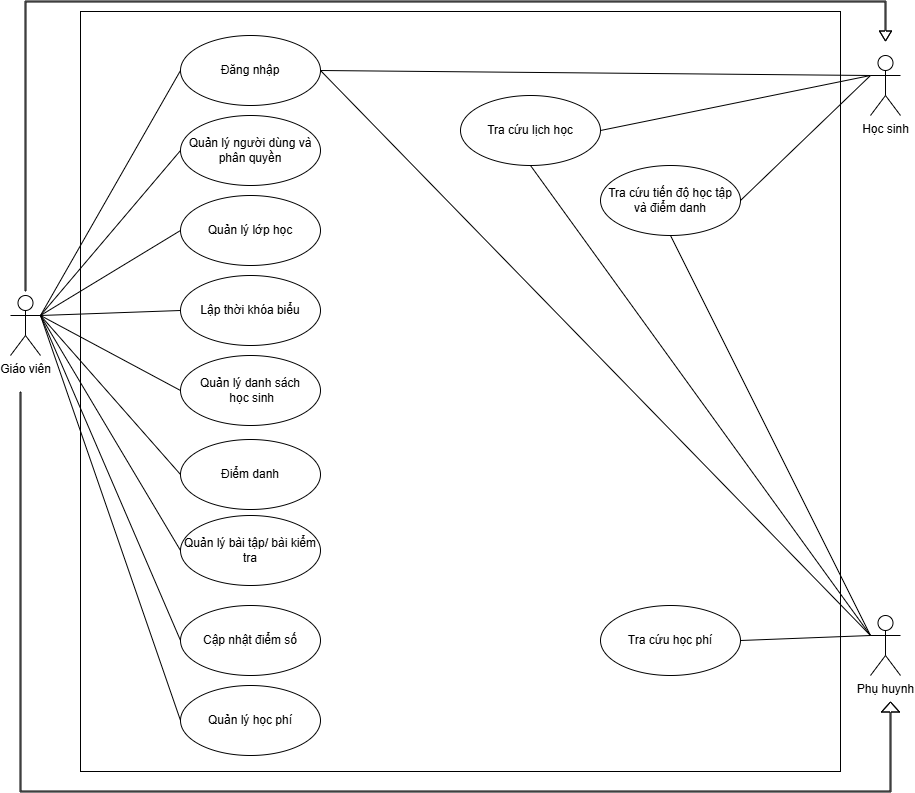
\includegraphics[width=1.0\textwidth]{picC2/UC_Tongquan.png}
    \caption{Sơ đồ use case tổng quan}
\end{figure}
\clearpage
\subsection{Biểu đồ use case phân rã mức 2}
\begin{figure}[htbp]
    \centering
    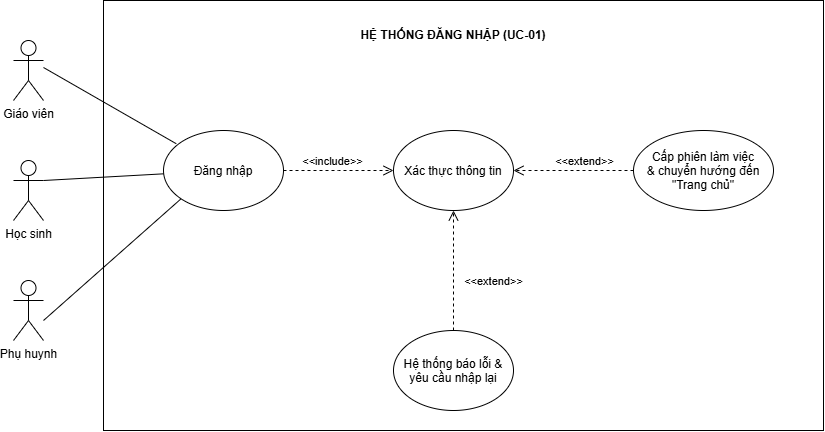
\includegraphics[width=1.0\textwidth]{picC2/UC1.png}
    \caption{Sơ đồ use case UC-01}
\end{figure}

\begin{figure}[htbp]
    \centering
    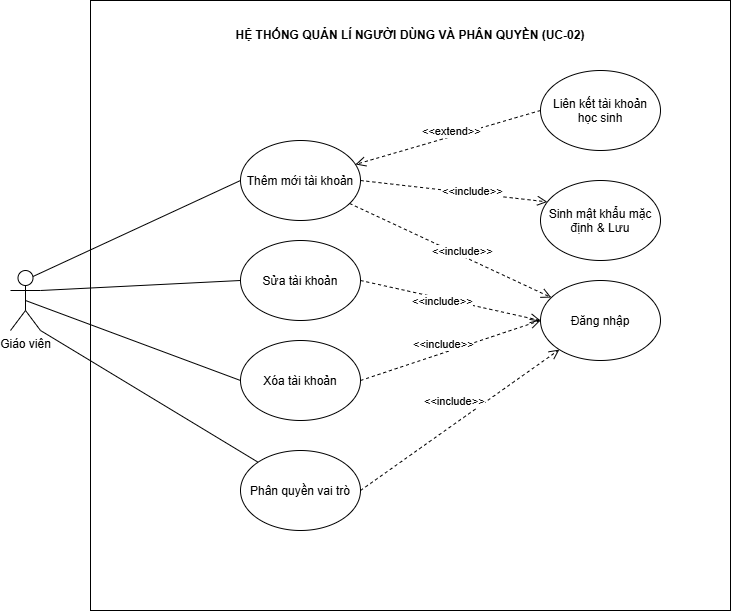
\includegraphics[width=1.0\textwidth]{picC2/UC2.png}
    \caption{Sơ đồ use case UC-02}
\end{figure}

\begin{figure}[htbp]
    \centering
    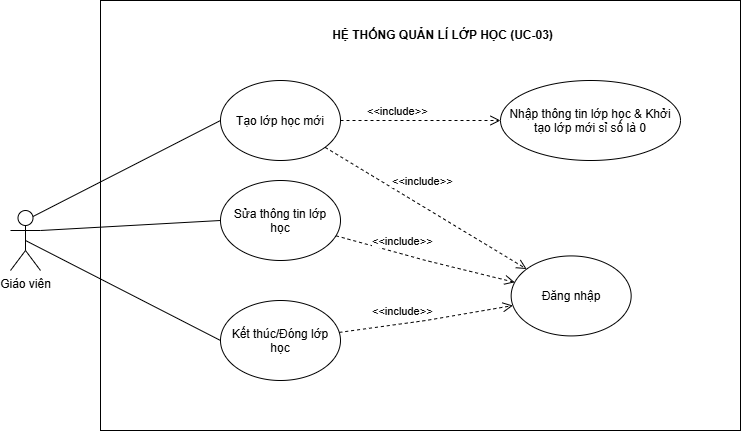
\includegraphics[width=1.0\textwidth]{picC2/UC3.png}
    \caption{Sơ đồ use case UC-03}
\end{figure}

\begin{figure}[htbp]
    \centering
    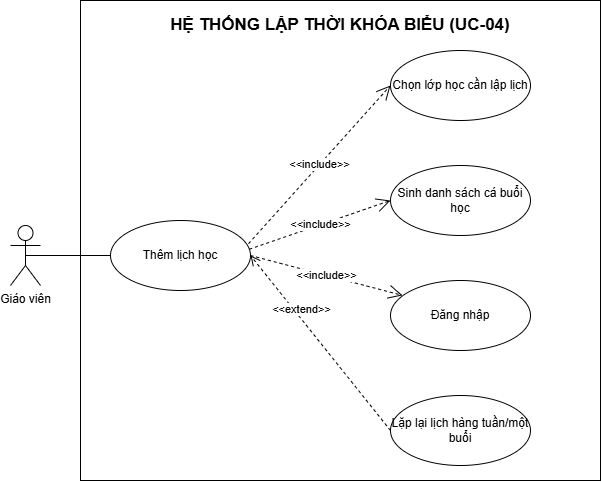
\includegraphics[width=1.0\textwidth]{picC2/UC4.png}
    \caption{Sơ đồ use case UC-04}
\end{figure}

\begin{figure}[htbp]
    \centering
    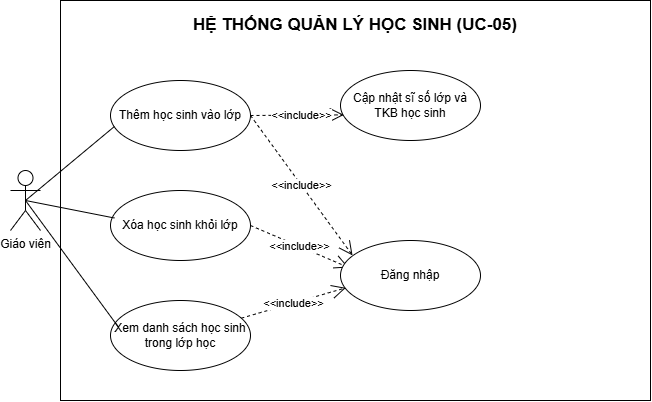
\includegraphics[width=1.0\textwidth]{picC2/UC5.png}
    \caption{Sơ đồ use case UC-05}
\end{figure}

\begin{figure}[htbp]
    \centering
    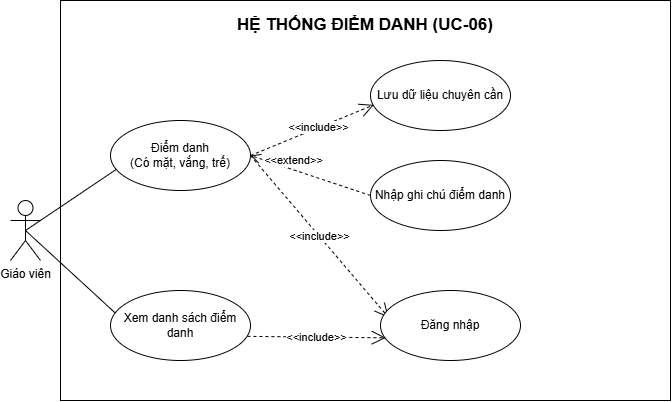
\includegraphics[width=1.0\textwidth]{picC2/UC6.png}
    \caption{Sơ đồ use case UC-06}
\end{figure}

\begin{figure}[htbp]
    \centering
    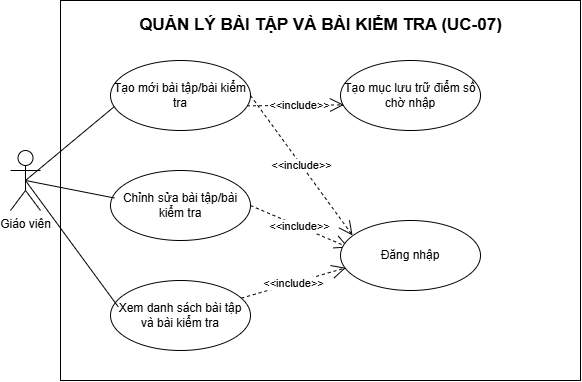
\includegraphics[width=1.0\textwidth]{picC2/UC7.png}
    \caption{Sơ đồ use case UC-07}
\end{figure}

\begin{figure}[htbp]
    \centering
    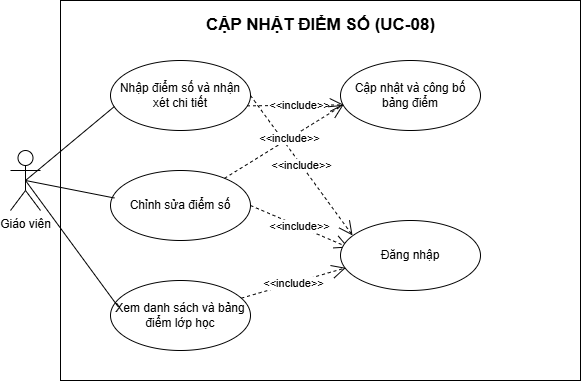
\includegraphics[width=1.0\textwidth]{picC2/UC8.png}
    \caption{Sơ đồ use case UC-08}
\end{figure}

\begin{figure}[htbp]
    \centering
    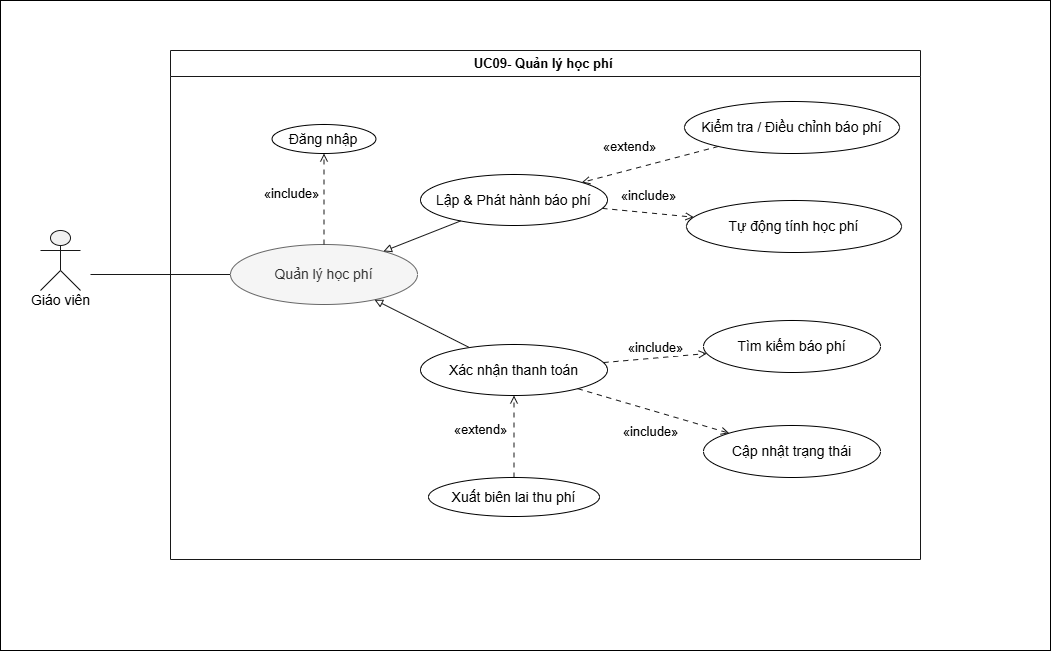
\includegraphics[width=1.0\textwidth]{picC2/UC9.png}
    \caption{Sơ đồ use case UC-09}
\end{figure}

\begin{figure}[htbp]
    \centering
    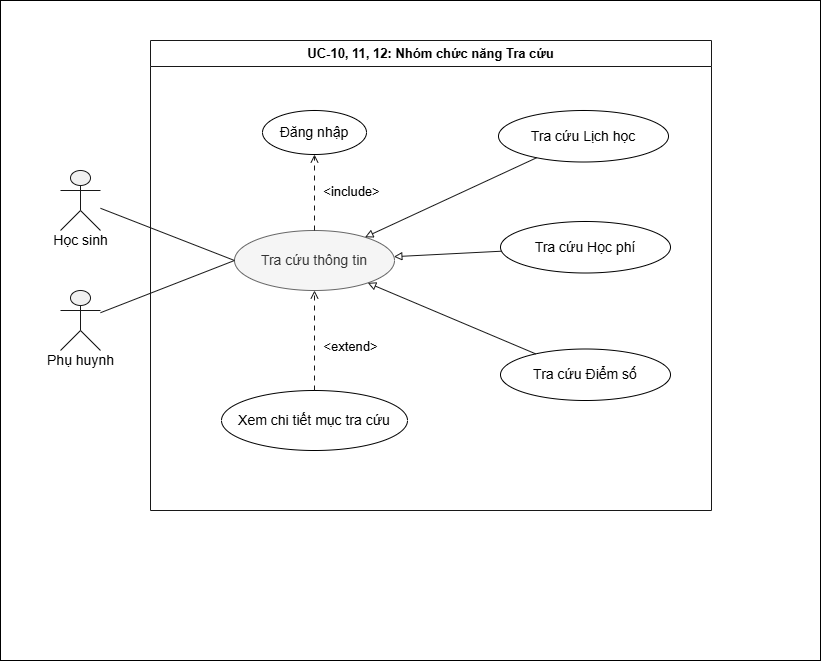
\includegraphics[width=1.0\textwidth]{picC2/UC10,11,12.png}
    \caption{Sơ đồ use case UC-10, UC-11, UC-12}
\end{figure}
\clearpage
\section{Biểu đồ hoạt động}

\subsection{AD-01: Quy trình Đăng nhập hệ thống (UC-01)}
\textbf{Mục đích:} Đặc tả luồng xác thực người dùng. Đây là cổng bảo mật đầu tiên, có rẽ nhánh logic để xử lý đúng/sai mật khẩu và chuyển hướng giao diện tùy thuộc vào vai trò của Actor.

\textbf{Mô tả:} Người dùng nhập thông tin đăng nhập. Hệ thống đối chiếu cơ sở dữ liệu. Nếu sai, hệ thống báo lỗi và quay lại nút kết hợp để yêu cầu nhập lại. Nếu đúng, hệ thống khởi tạo phiên làm việc (Session), kiểm tra vai trò (Giáo viên, Học sinh, Phụ huynh) và điều hướng đến Dashboard tương ứng.

\begin{figure}[htbp]
    \centering
    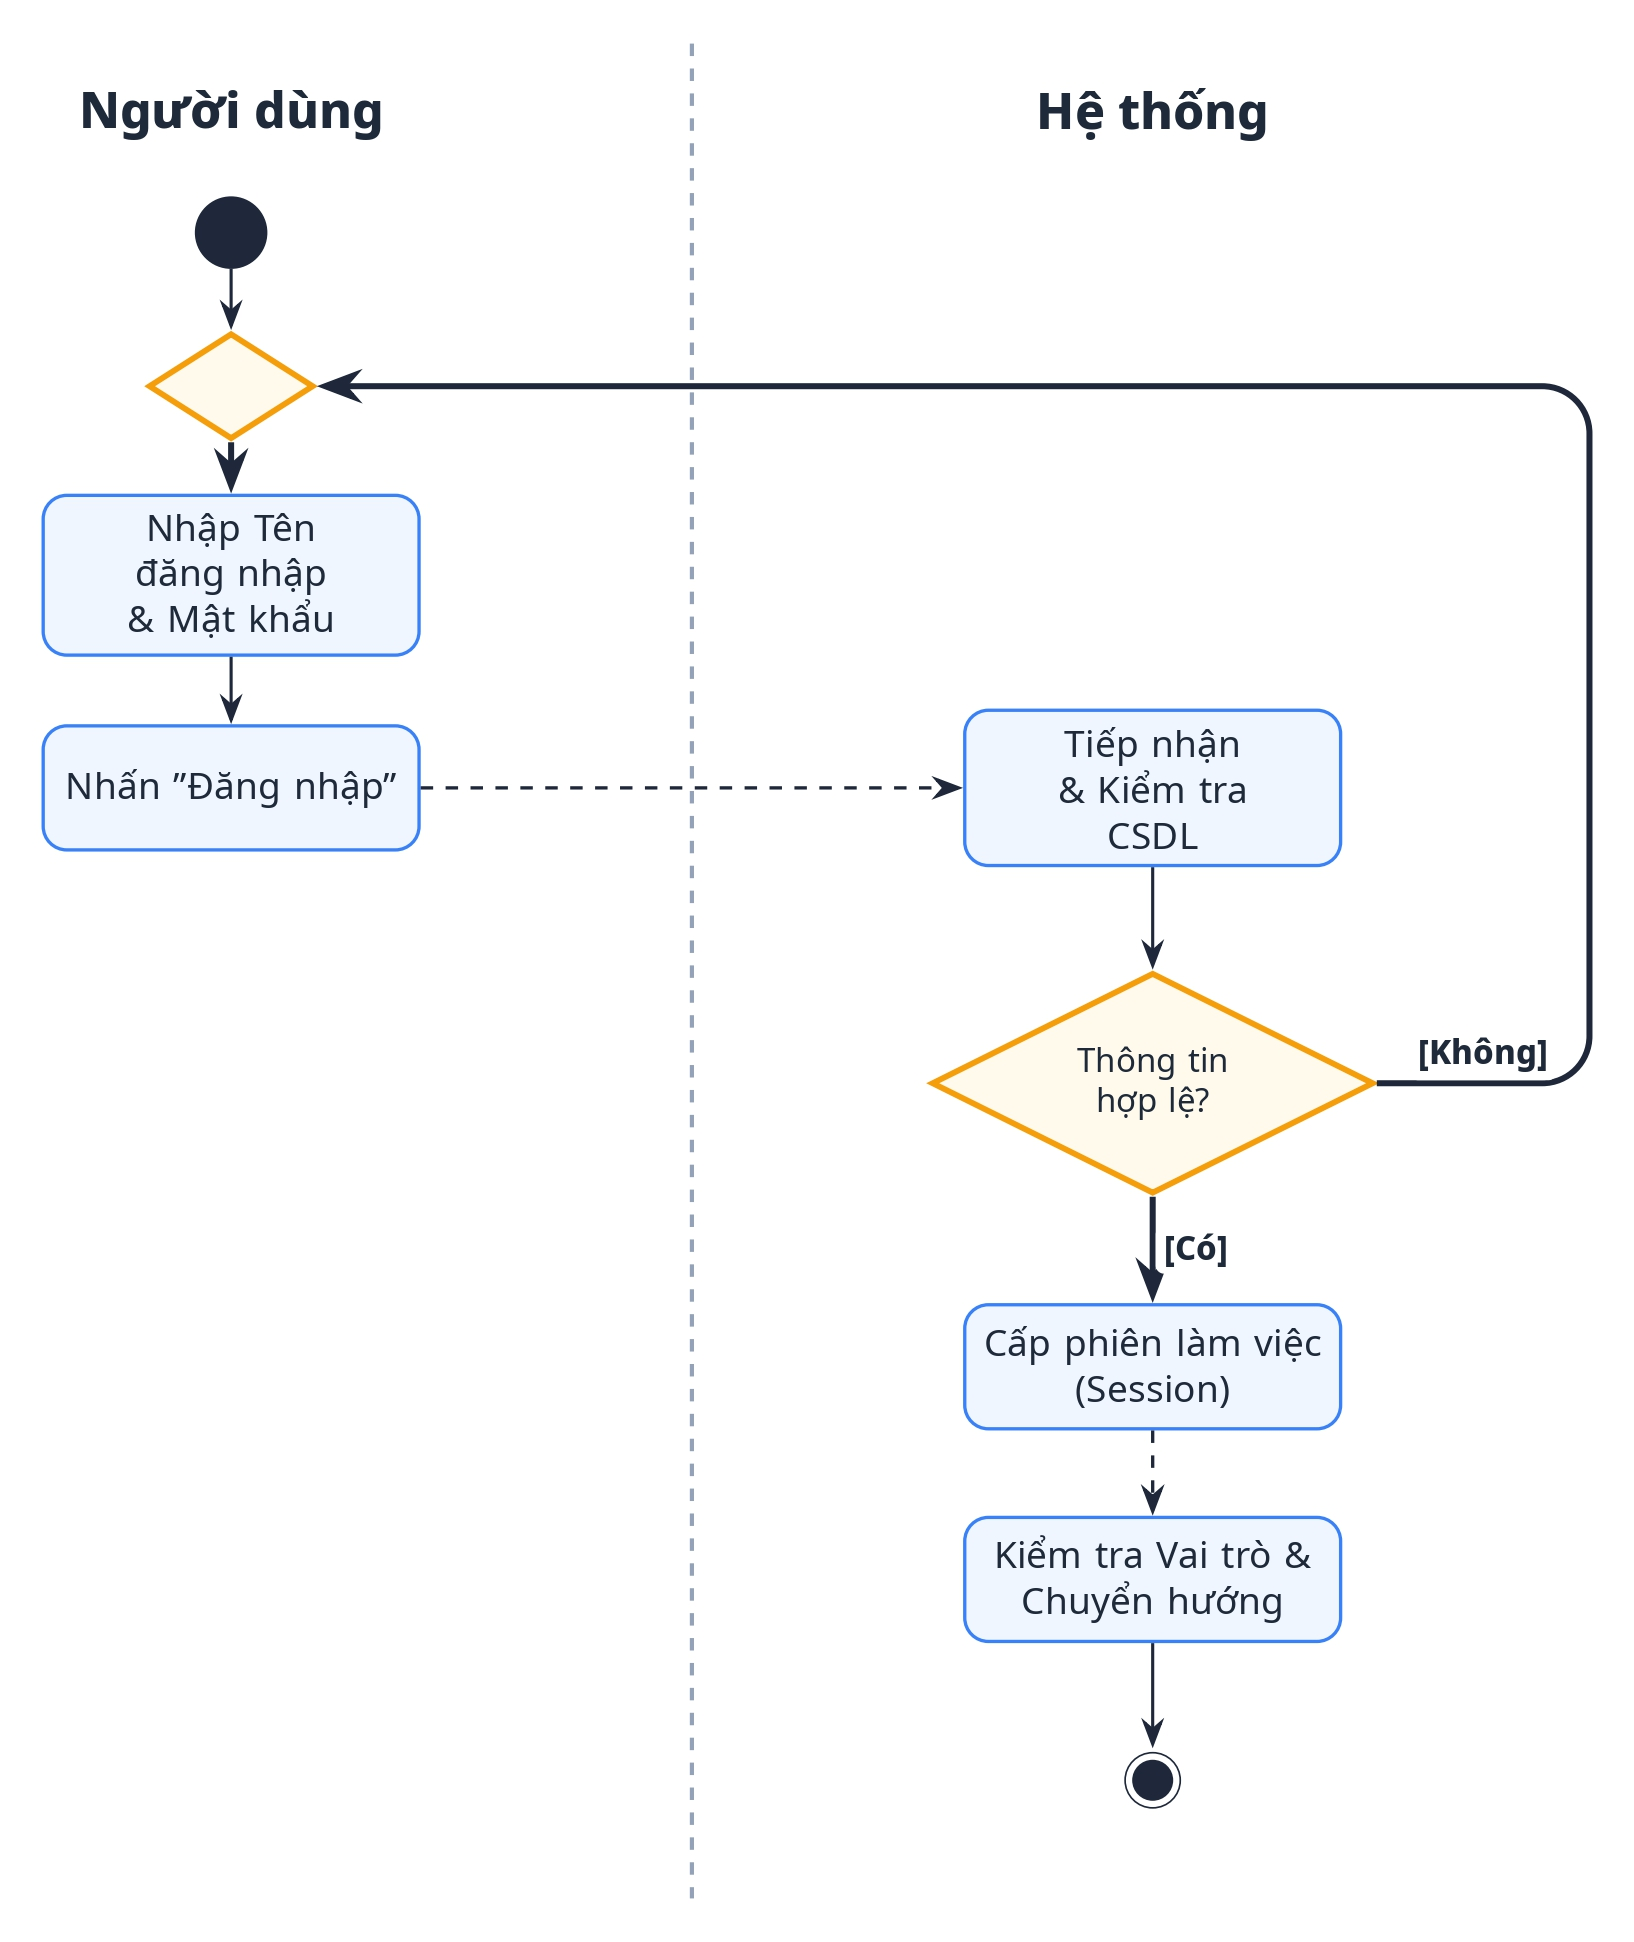
\includegraphics[width=0.8\textwidth]{picC2/AD1.jpg}
    \caption{AD-01: Quy trình Đăng nhập hệ thống}
\end{figure}

\clearpage

\subsection{AD-02: Quy trình Tạo mới và Phân quyền (UC-02)}
\textbf{Mục đích:} Đặc tả các bước giáo viên tạo tài khoản cho học sinh và phụ huynh.

\textbf{Mô tả:} Giáo viên nhập thông tin cơ bản và chọn vai trò. Nếu chọn "Phụ huynh", hệ thống sẽ bắt buộc yêu cầu chọn liên kết với một tài khoản Học sinh đang có. Hai nhánh xử lý hội tụ tại nút kết hợp trước khi nhấn "Lưu", sau đó hệ thống sinh tài khoản, tạo mật khẩu mặc định và lưu vào CSDL.

\begin{figure}[htbp]
    \centering
    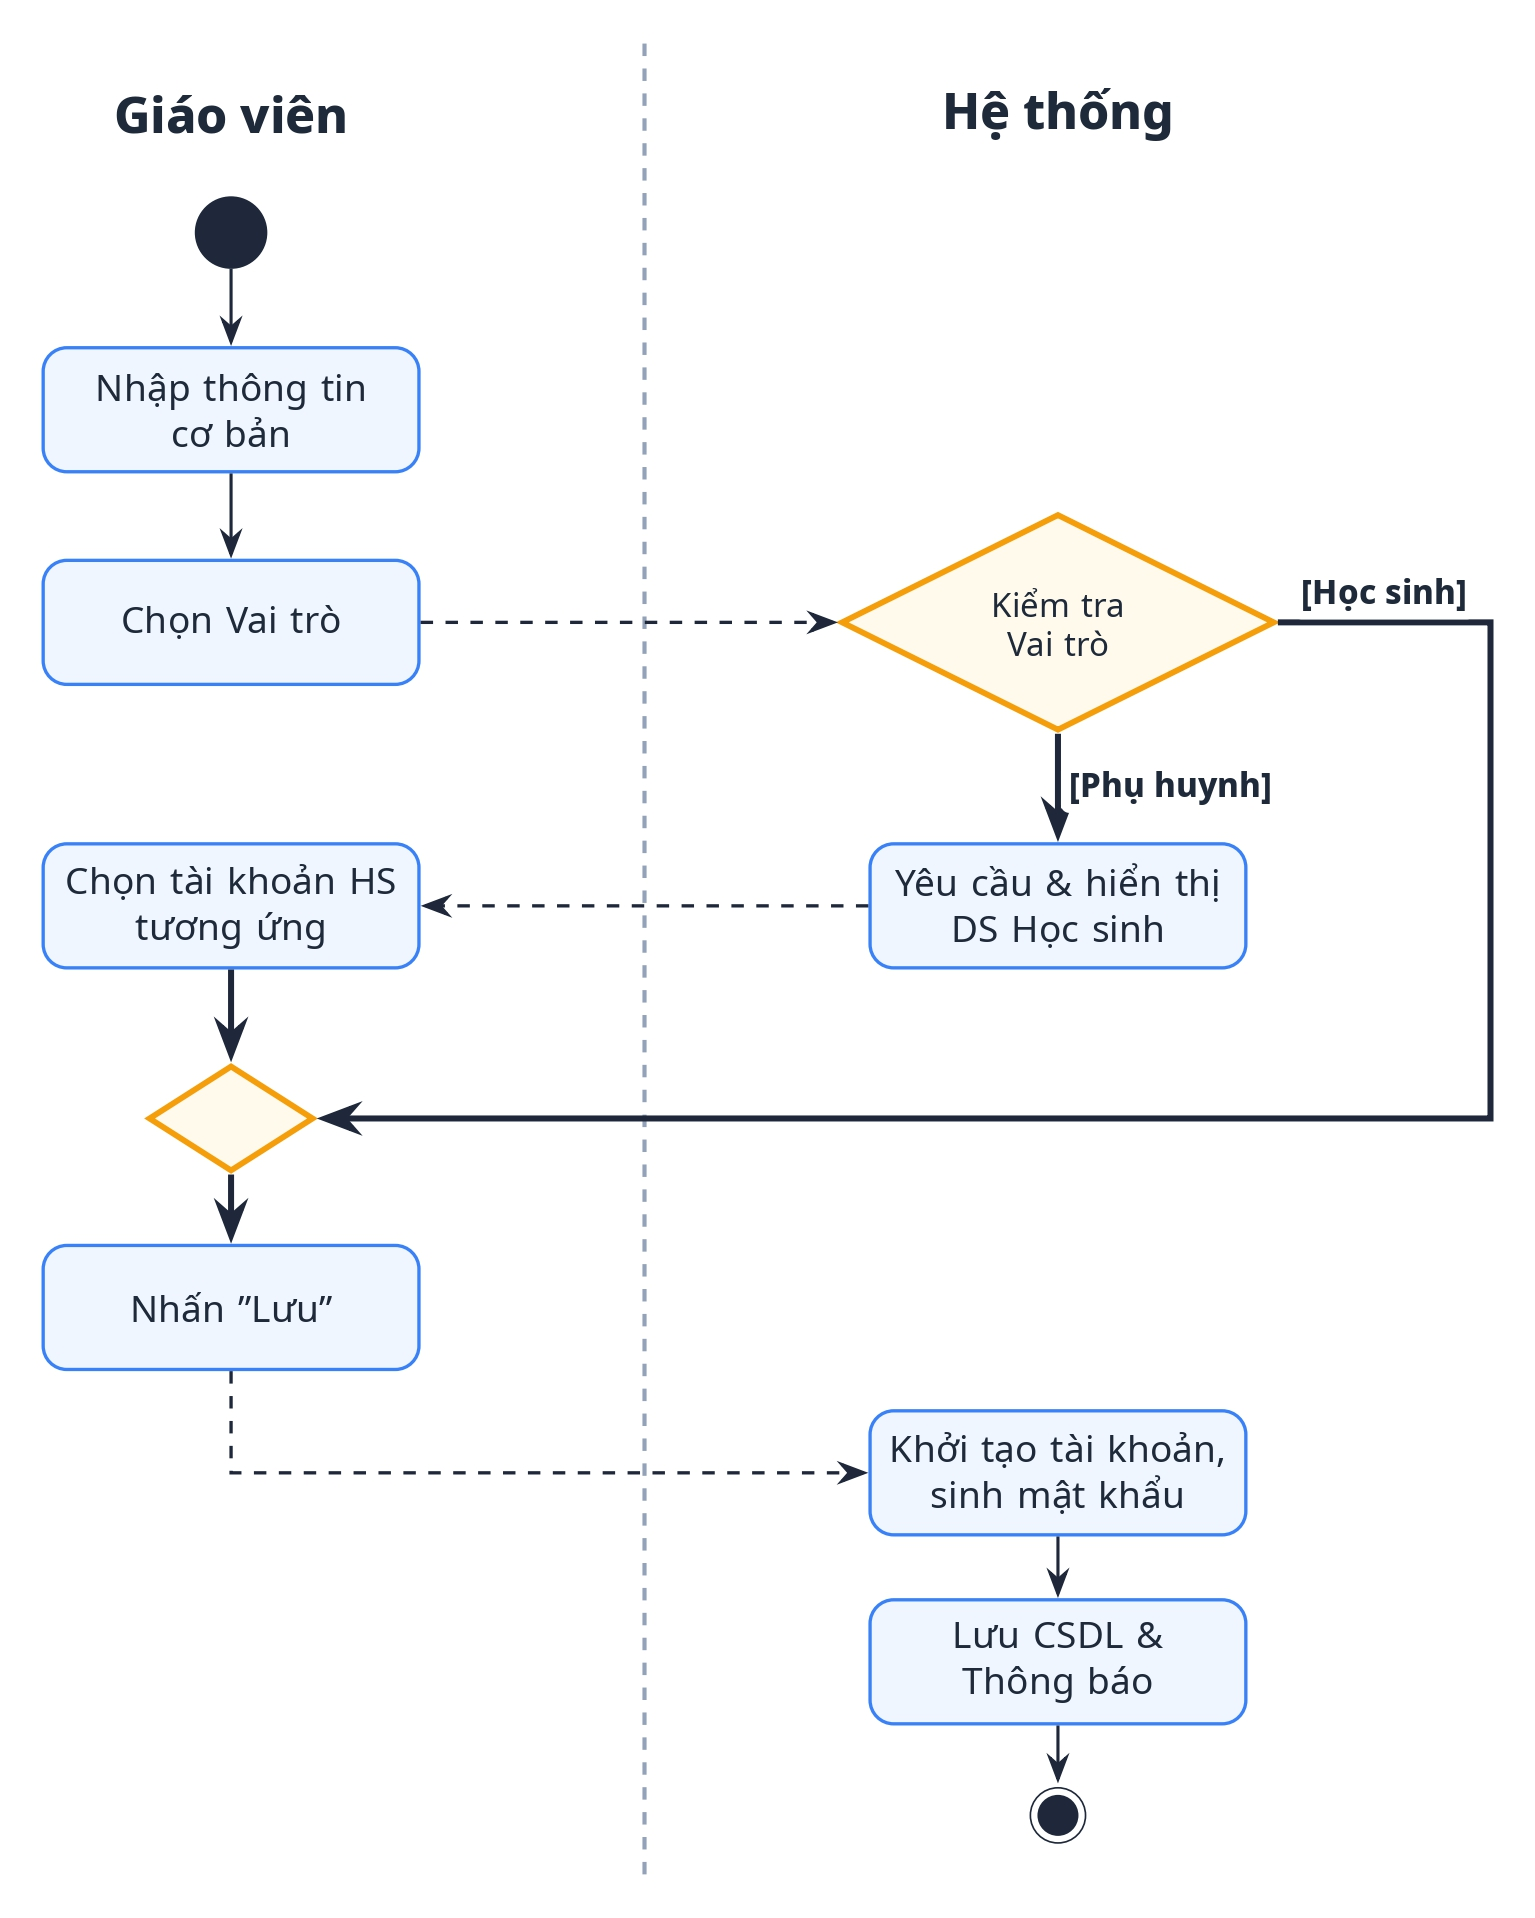
\includegraphics[width=0.8\textwidth]{picC2/AD2.jpg}
    \caption{AD-02: Quy trình Tạo mới và Phân quyền}
\end{figure}

\clearpage

\subsection{AD-03: Quy trình Khởi tạo và Thiết lập Lớp học (UC-03, 04, 05)}
\textbf{Mục đích:} Thể hiện chuỗi hành động liên kết tuần tự để một lớp học có thể vận hành.

\textbf{Mô tả:} Việc thiết lập lớp học yêu cầu 3 giai đoạn chặt chẽ: Đầu tiên, giáo viên tạo thông tin khung của lớp. Tiếp theo, giáo viên thêm danh sách học sinh để hệ thống cập nhật sĩ số. Cuối cùng, giáo viên lên lịch học (một buổi hoặc lặp lại theo chu kỳ định kỳ) và hệ thống đồng bộ lịch này vào thời khóa biểu của từng học sinh.

\begin{figure}[htbp]
    \centering
    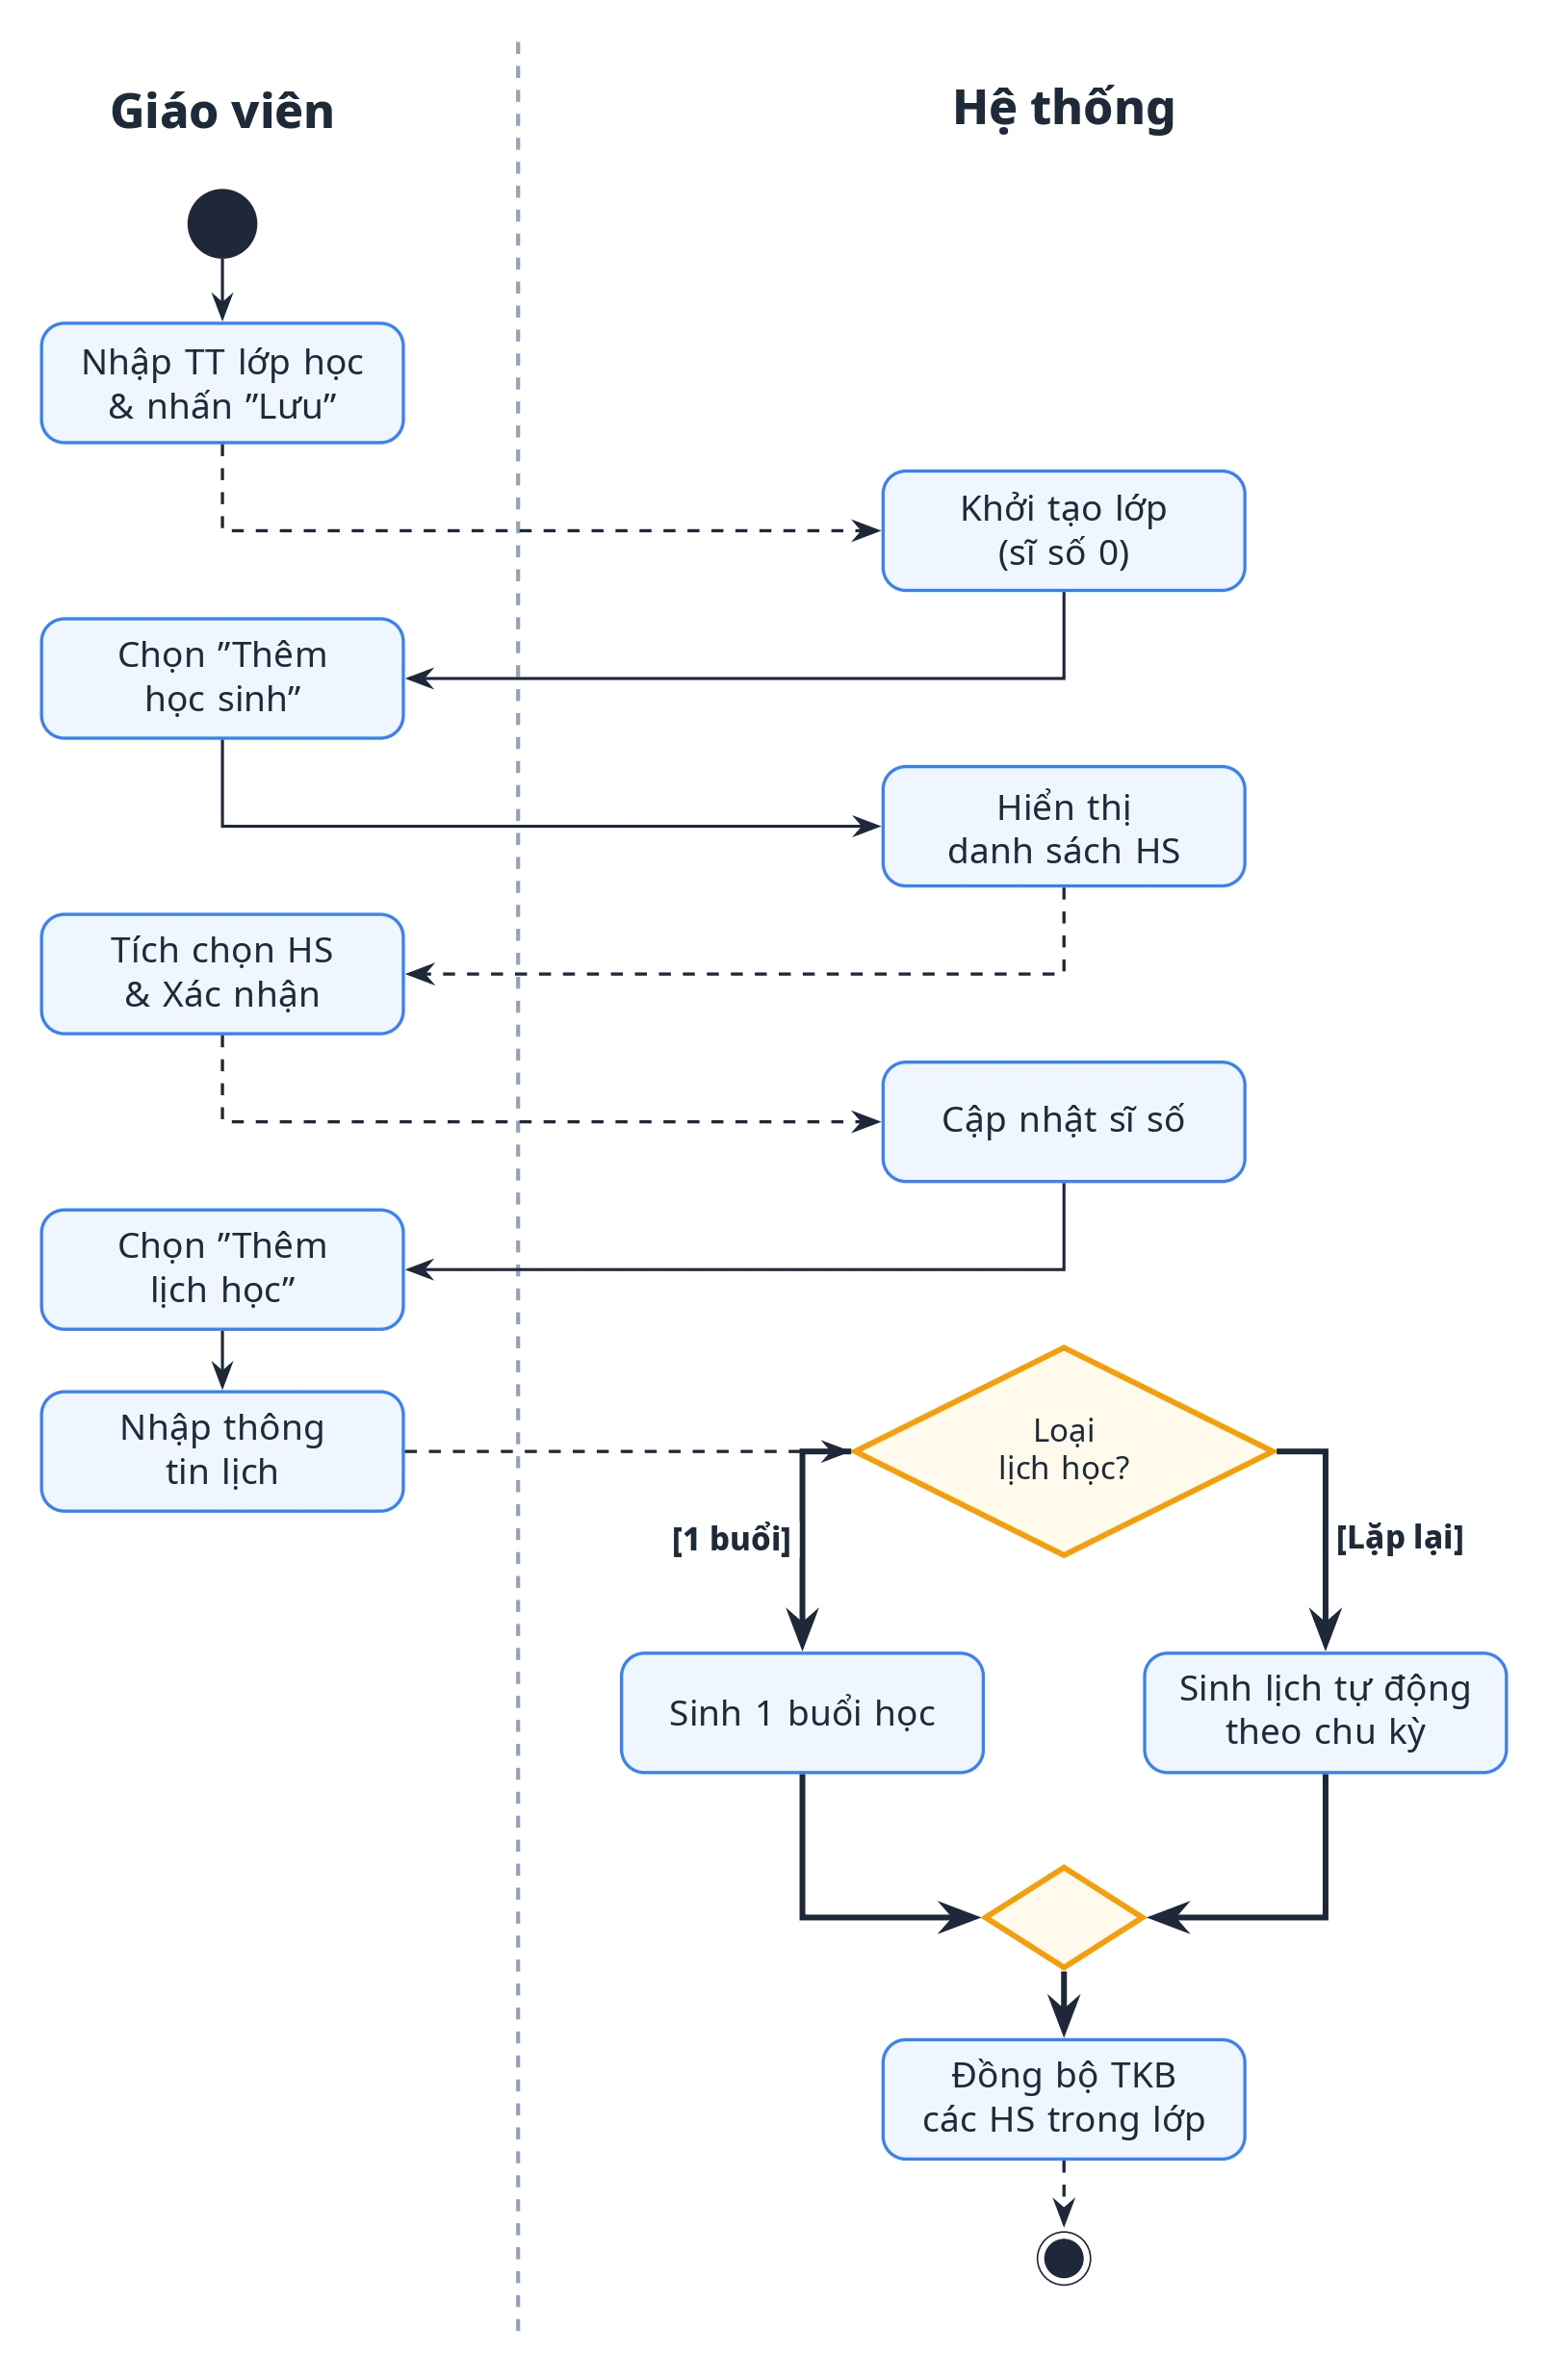
\includegraphics[width=0.8\textwidth]{picC2/AD3.jpg}
    \caption{AD-03: Quy trình Khởi tạo và Thiết lập Lớp học}
\end{figure}

\clearpage

\subsection{AD-04: Quy trình Điểm danh buổi học (UC-06)}
\textbf{Mục đích:} Ghi nhận chuyên cần của lớp học.

\textbf{Mô tả:} Giáo viên kích hoạt chức năng điểm danh. Hệ thống hiển thị danh sách học sinh. Giáo viên thực hiện vòng lặp kiểm tra và đánh dấu trạng thái (Có mặt / Vắng / Trễ) kèm ghi chú cho từng học sinh. Sau khi duyệt hết danh sách, giáo viên lưu dữ liệu để hệ thống ghi nhận vào CSDL.

\begin{figure}[htbp]
    \centering
    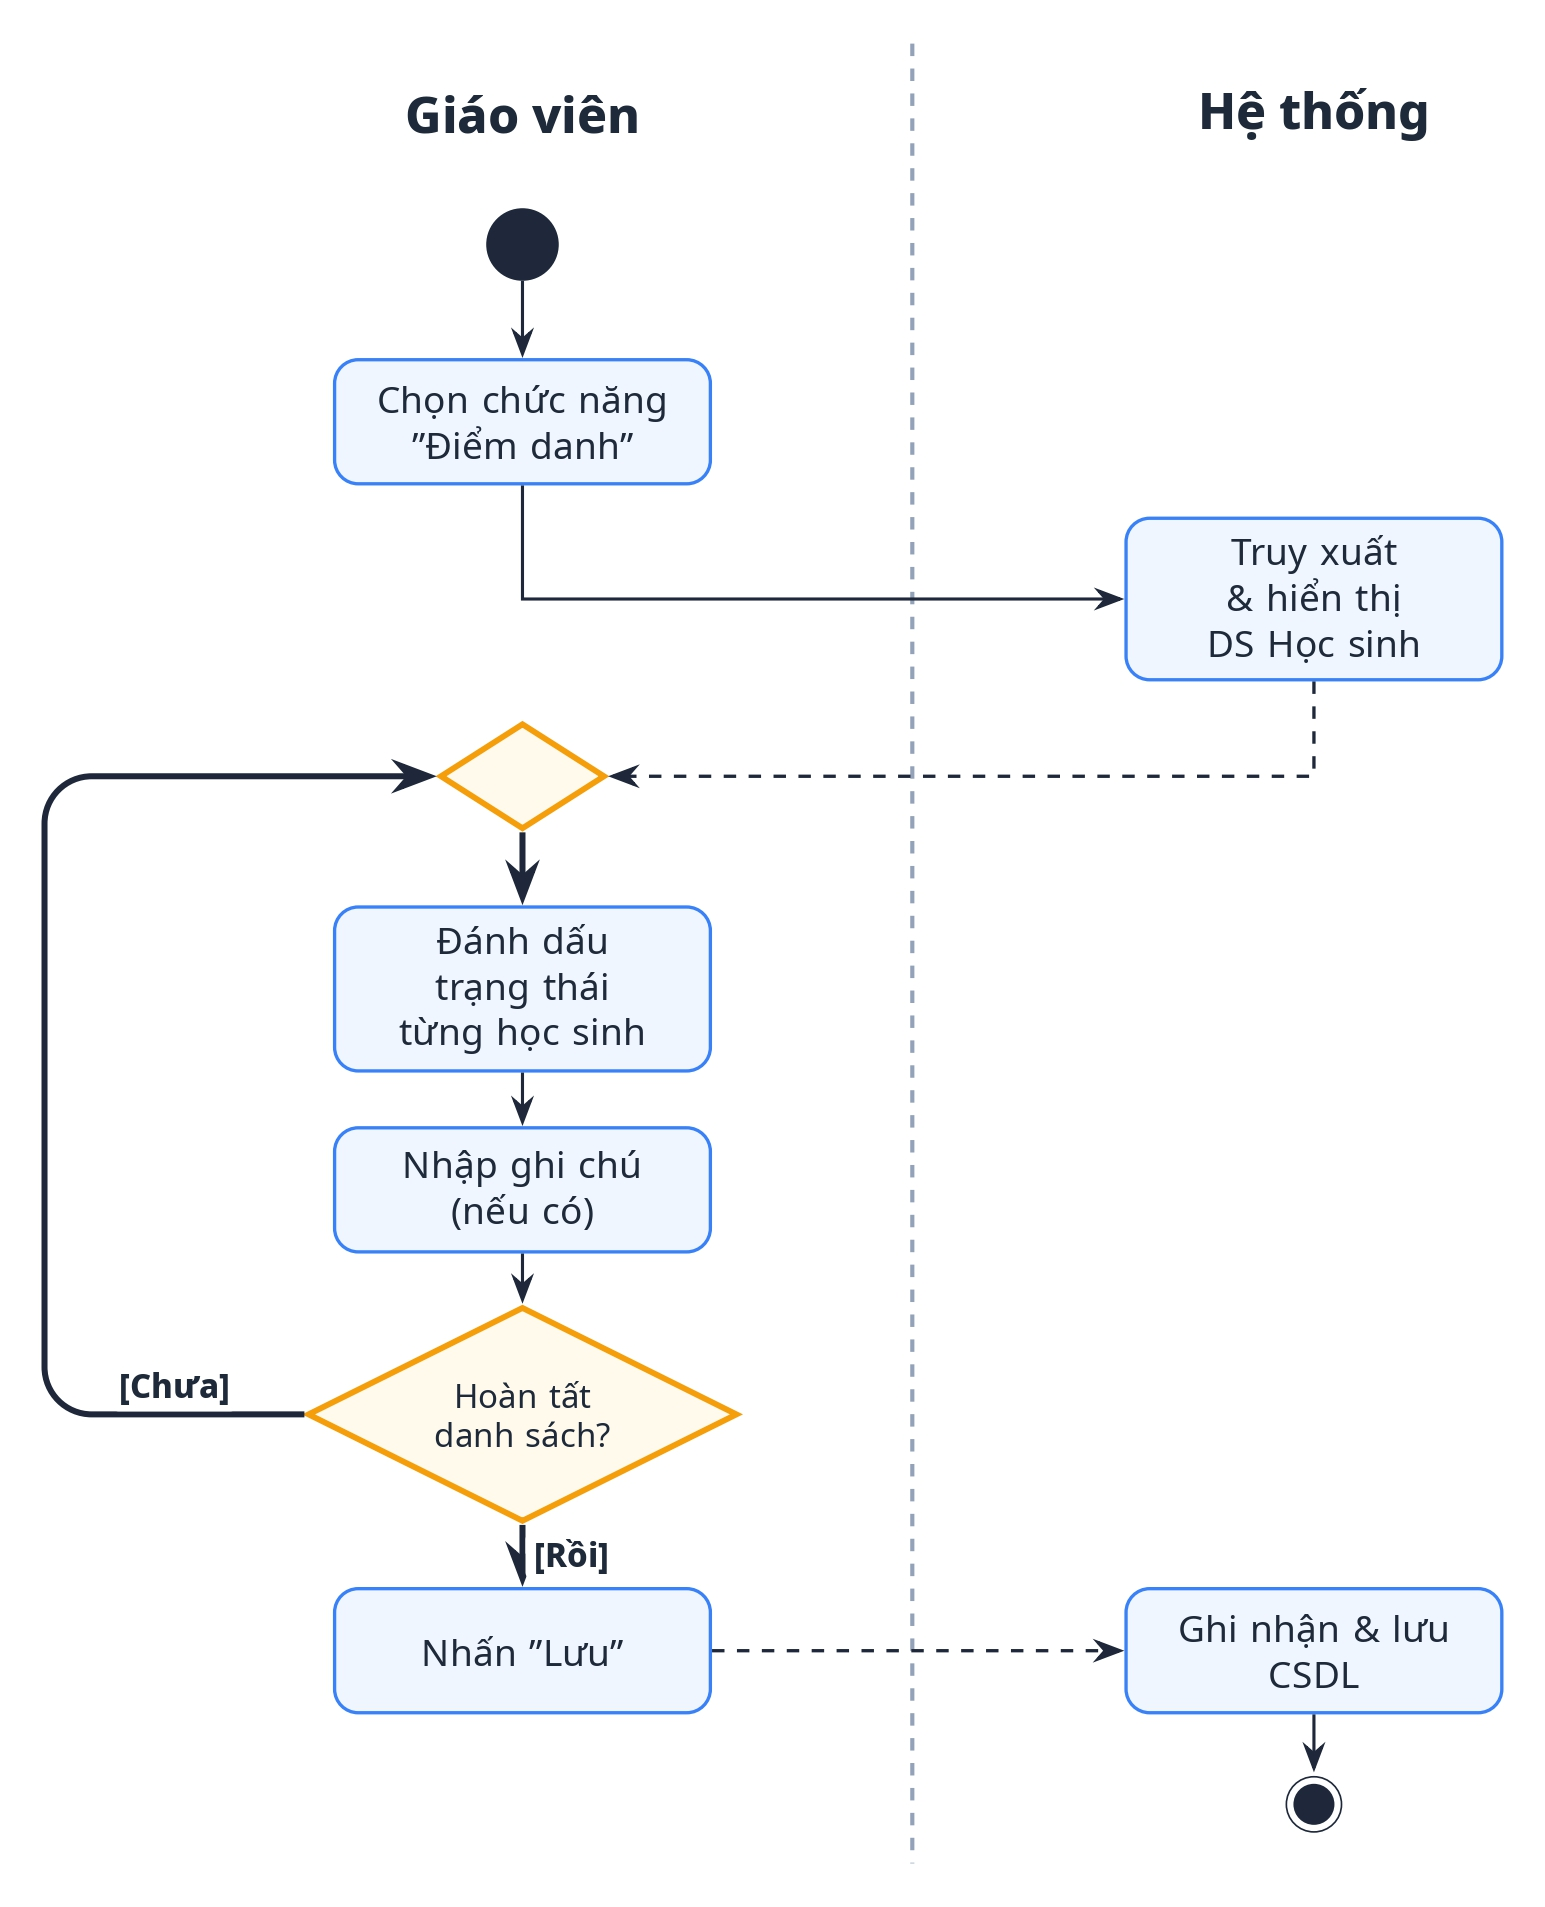
\includegraphics[width=0.8\textwidth]{picC2/AD4.jpg}
    \caption{AD-04: Quy trình Điểm danh buổi học}
\end{figure}

\clearpage

\subsection{AD-05: Quy trình Quản lý Đánh giá và Điểm (UC-07, 08)}
\textbf{Mục đích:} Đặc tả việc tạo bài kiểm tra và quy trình nhập điểm, thể hiện luồng dữ liệu liền mạch từ lúc Giáo viên khởi tạo đến khi điểm số hiển thị cho người học.

\textbf{Mô tả:} Giáo viên tạo bài đánh giá mới hoặc chọn bài đánh giá đã có để cập nhật. Khi cần chấm, giáo viên mở danh sách lớp và nhập/sửa điểm số cùng nhận xét cho từng học sinh qua một vòng lặp. Hoàn tất quá trình, hệ thống tự động cập nhật bảng điểm tổng. Nếu là thao tác sửa điểm cũ, hệ thống thực hiện "Lưu lịch sử chỉnh sửa điểm"; nếu là nhập điểm mới, hệ thống thực hiện "Lưu lịch sử nhập điểm".

\begin{figure}[htbp]
    \centering
    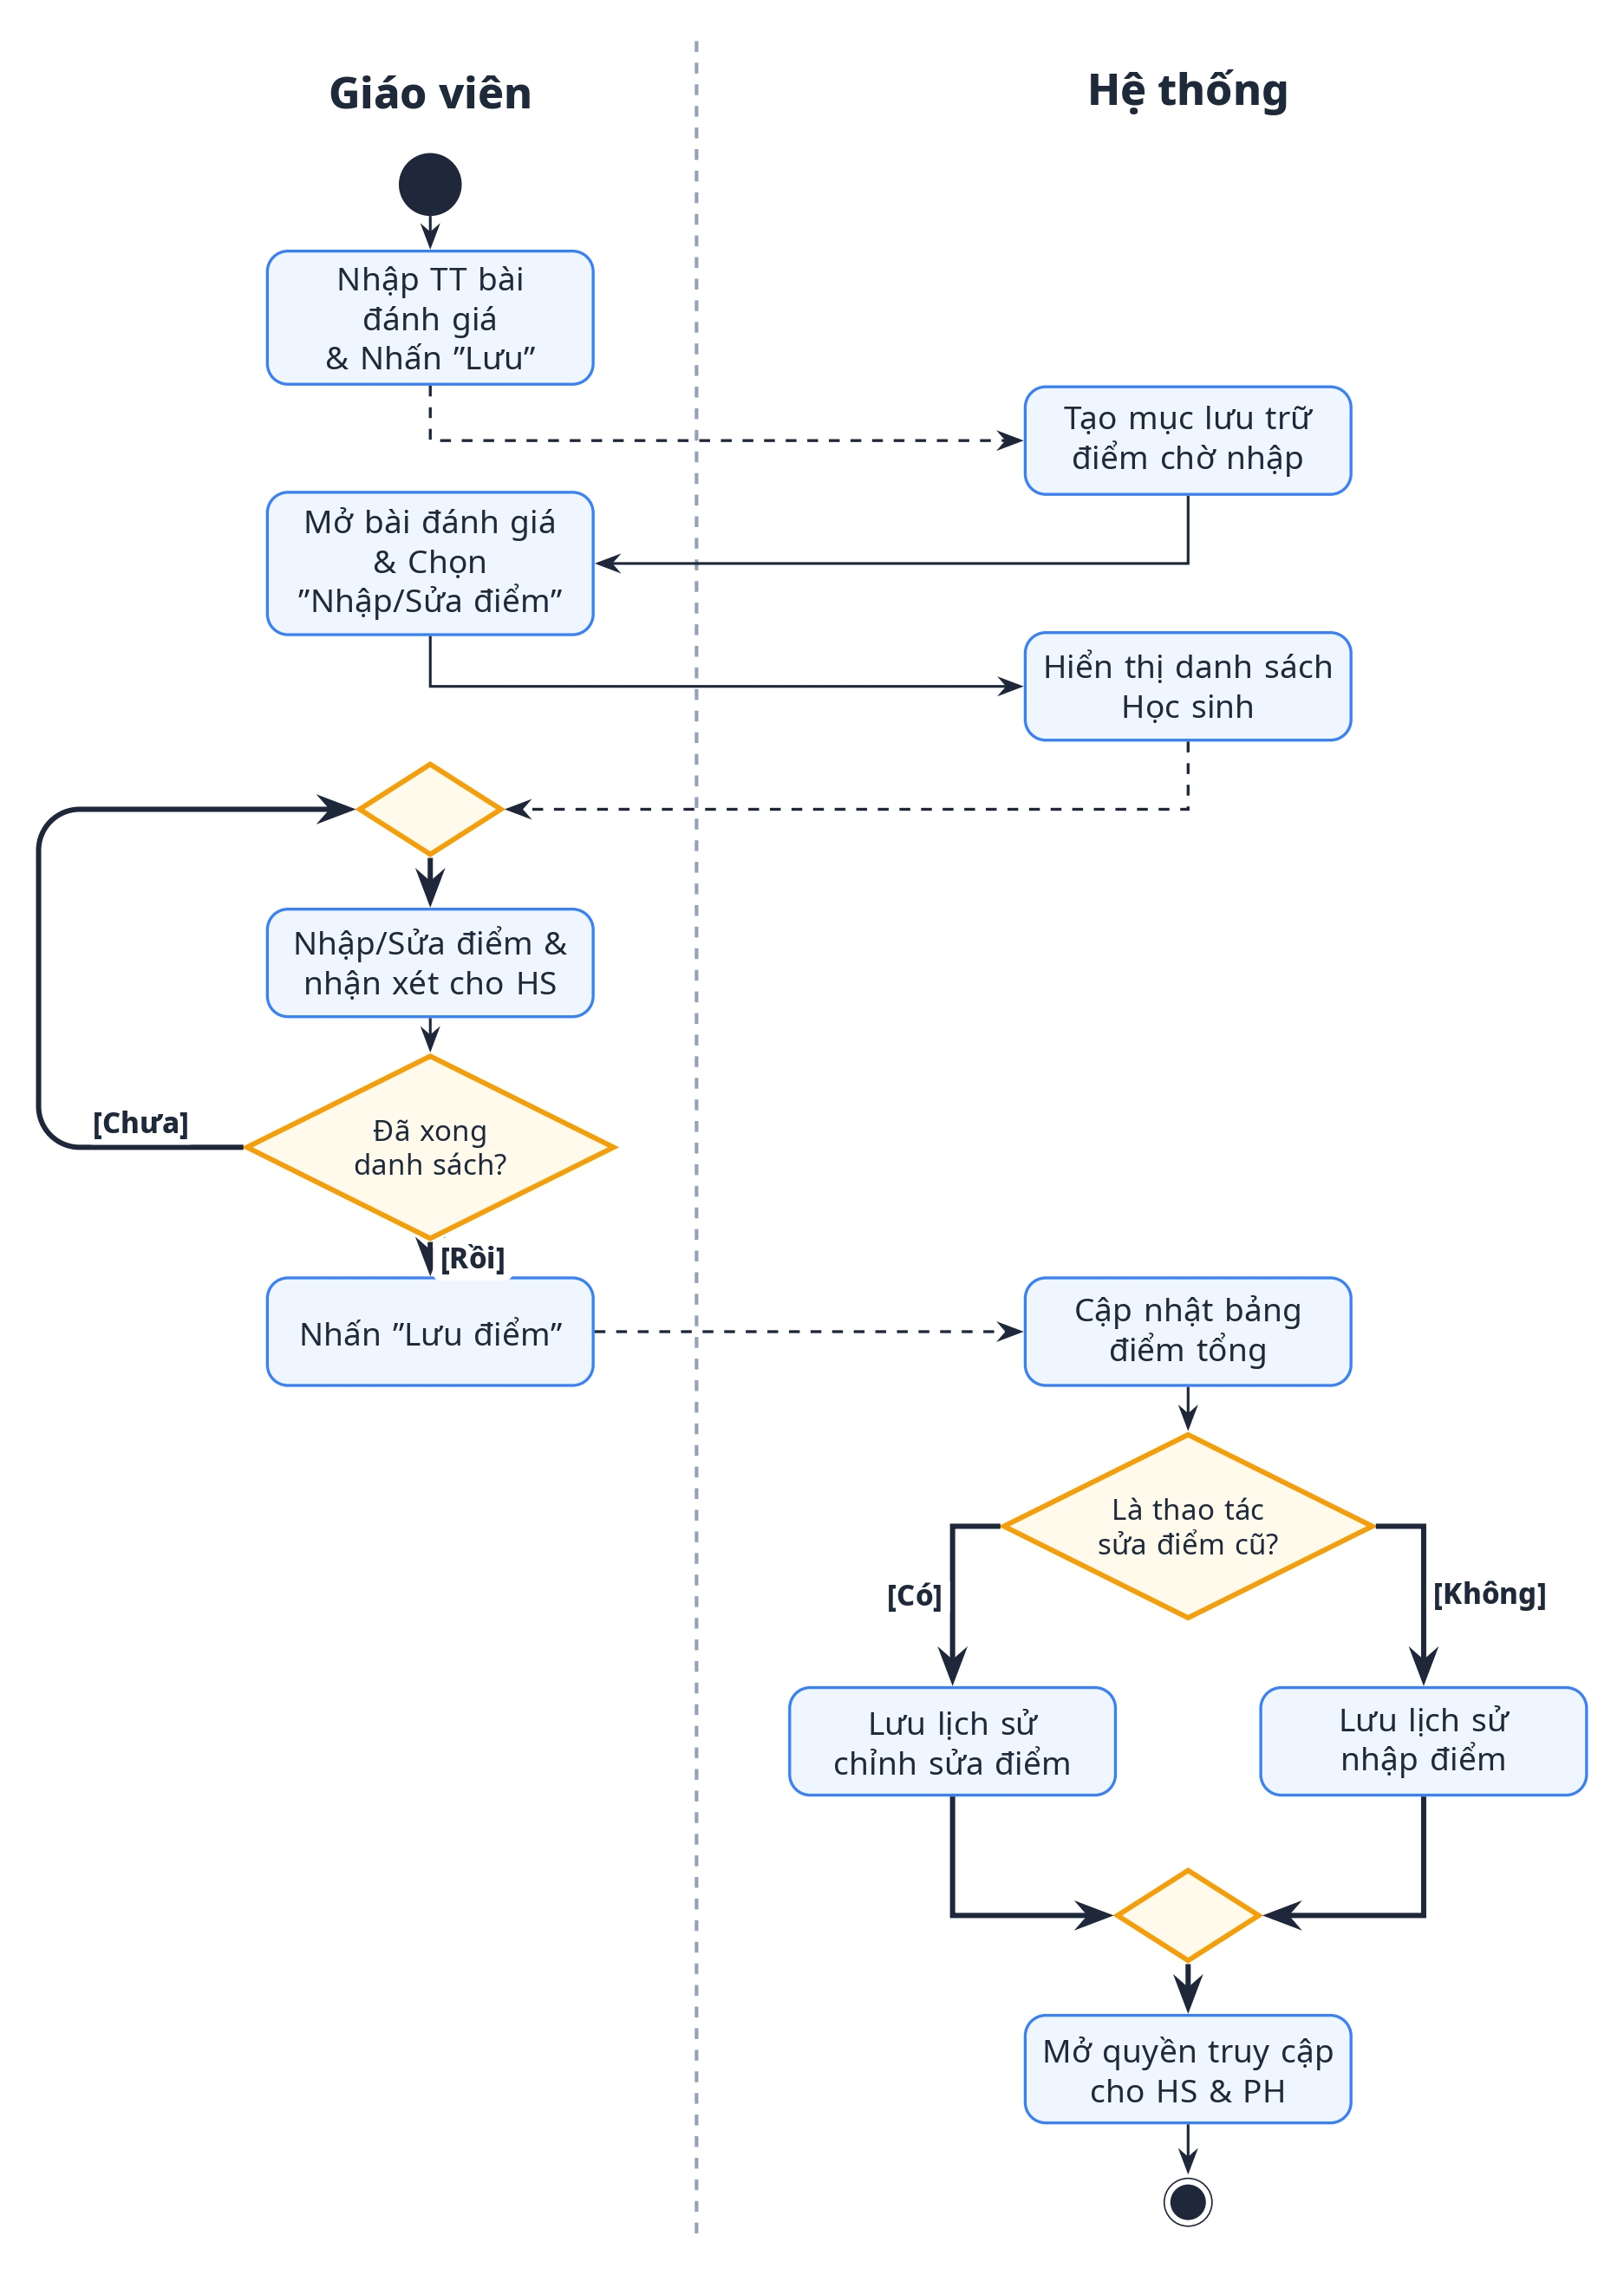
\includegraphics[width=0.8\textwidth]{picC2/AD5.jpg}
    \caption{AD-05: Quy trình Quản lý Đánh giá và Điểm}
\end{figure}

\clearpage

\subsection{AD-06: Quy trình Quản lý và Thu học phí (UC-09)}
\textbf{Mục đích:} Mô tả vòng đời của một hóa đơn học phí.

\textbf{Mô tả:} Hệ thống hỗ trợ tính toán tổng học phí tự động. Giáo viên kiểm duyệt và phát hành báo phí. Phụ huynh thực hiện chuyển khoản/đóng tiền mặt ngoài hệ thống. Giáo viên ghi nhận số tiền thực nhận trên hệ thống. Hệ thống đối chiếu số tiền này với tổng phí để cập nhật trạng thái "Đã đóng đủ" hoặc "Chưa đóng".

\begin{figure}[htbp]
\centering
    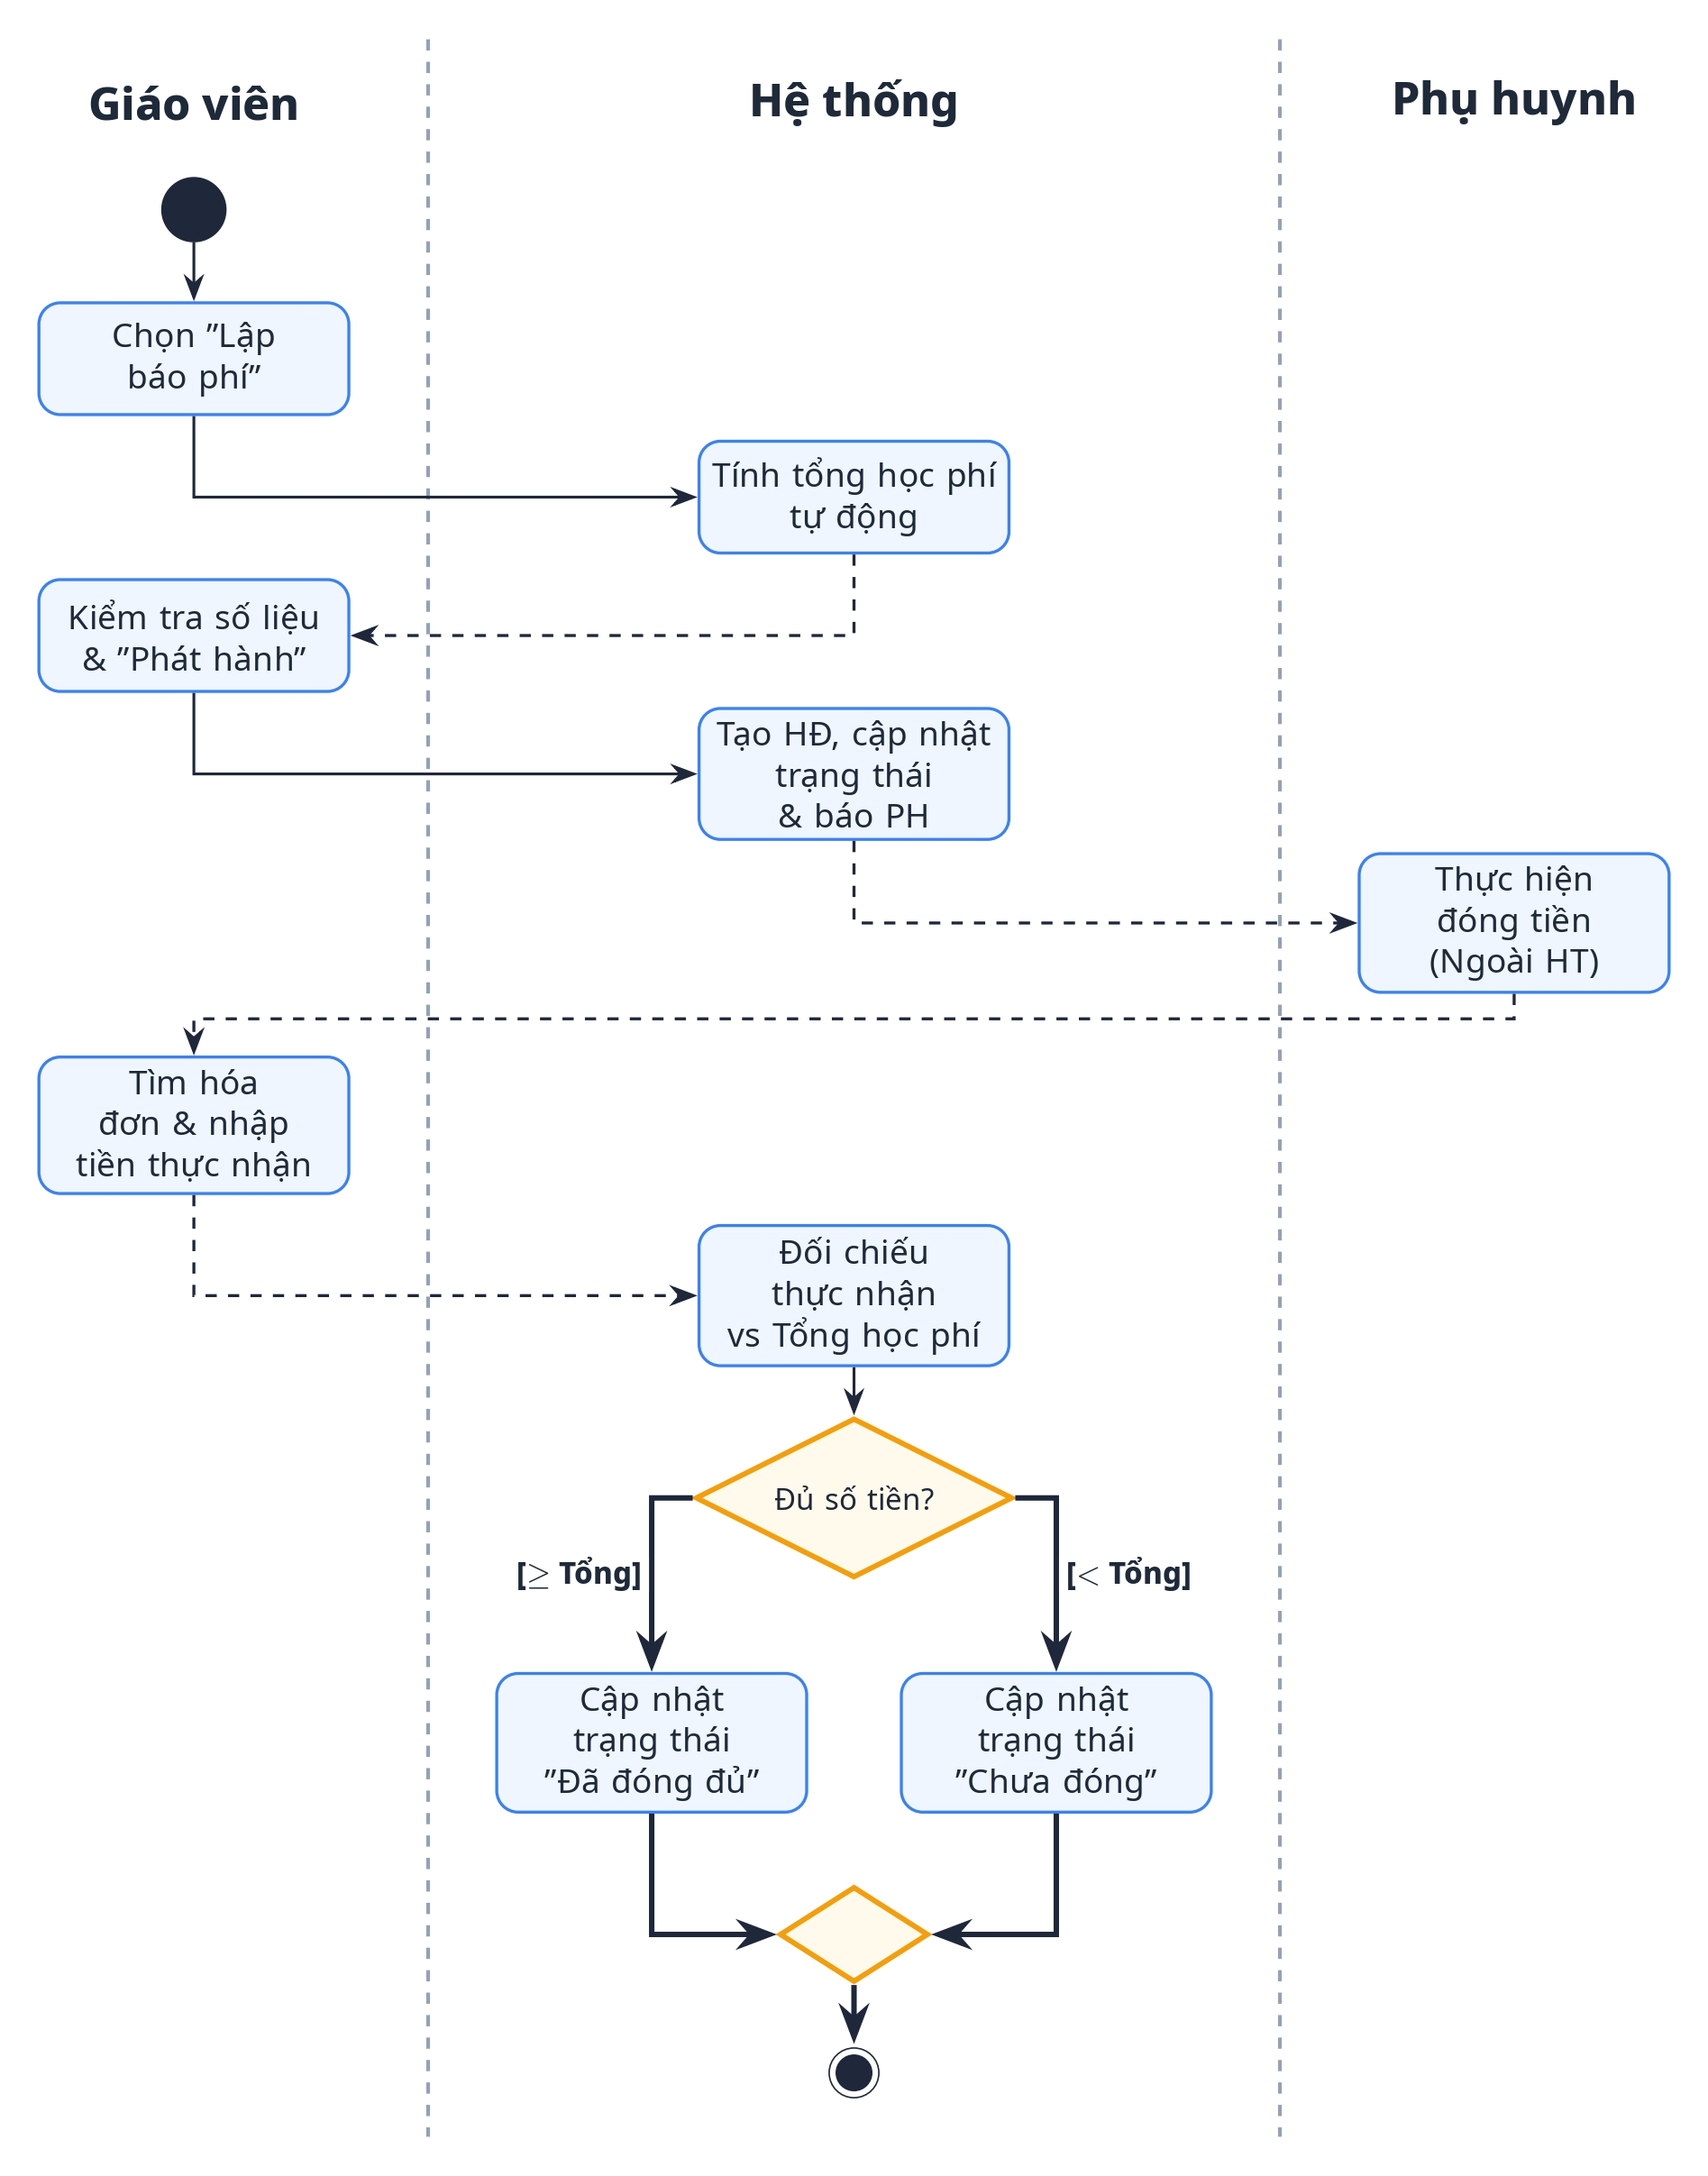
\includegraphics[width=0.8\textwidth]{picC2/AD6.jpg}
    \caption{AD-06: Quy trình Quản lý và Thu học phí}
\end{figure}

\clearpage

\subsection{AD-07: Quy trình Tra cứu thông tin (UC-10, 11, 12)}
\textbf{Mục đích:} Mô tả cách người dùng cuối tự phục vụ tra cứu thông tin cá nhân.

\textbf{Mô tả:} Người dùng chọn menu Tra cứu và lựa chọn danh mục mong muốn. Hệ thống rẽ nhánh truy xuất dữ liệu tương ứng (Thời khóa biểu, Điểm số, hoặc Hóa đơn) và hiển thị lên giao diện. Người dùng có thể nhấp vào từng mục cụ thể để xem chi tiết.

\begin{figure}[htbp]
\centering
    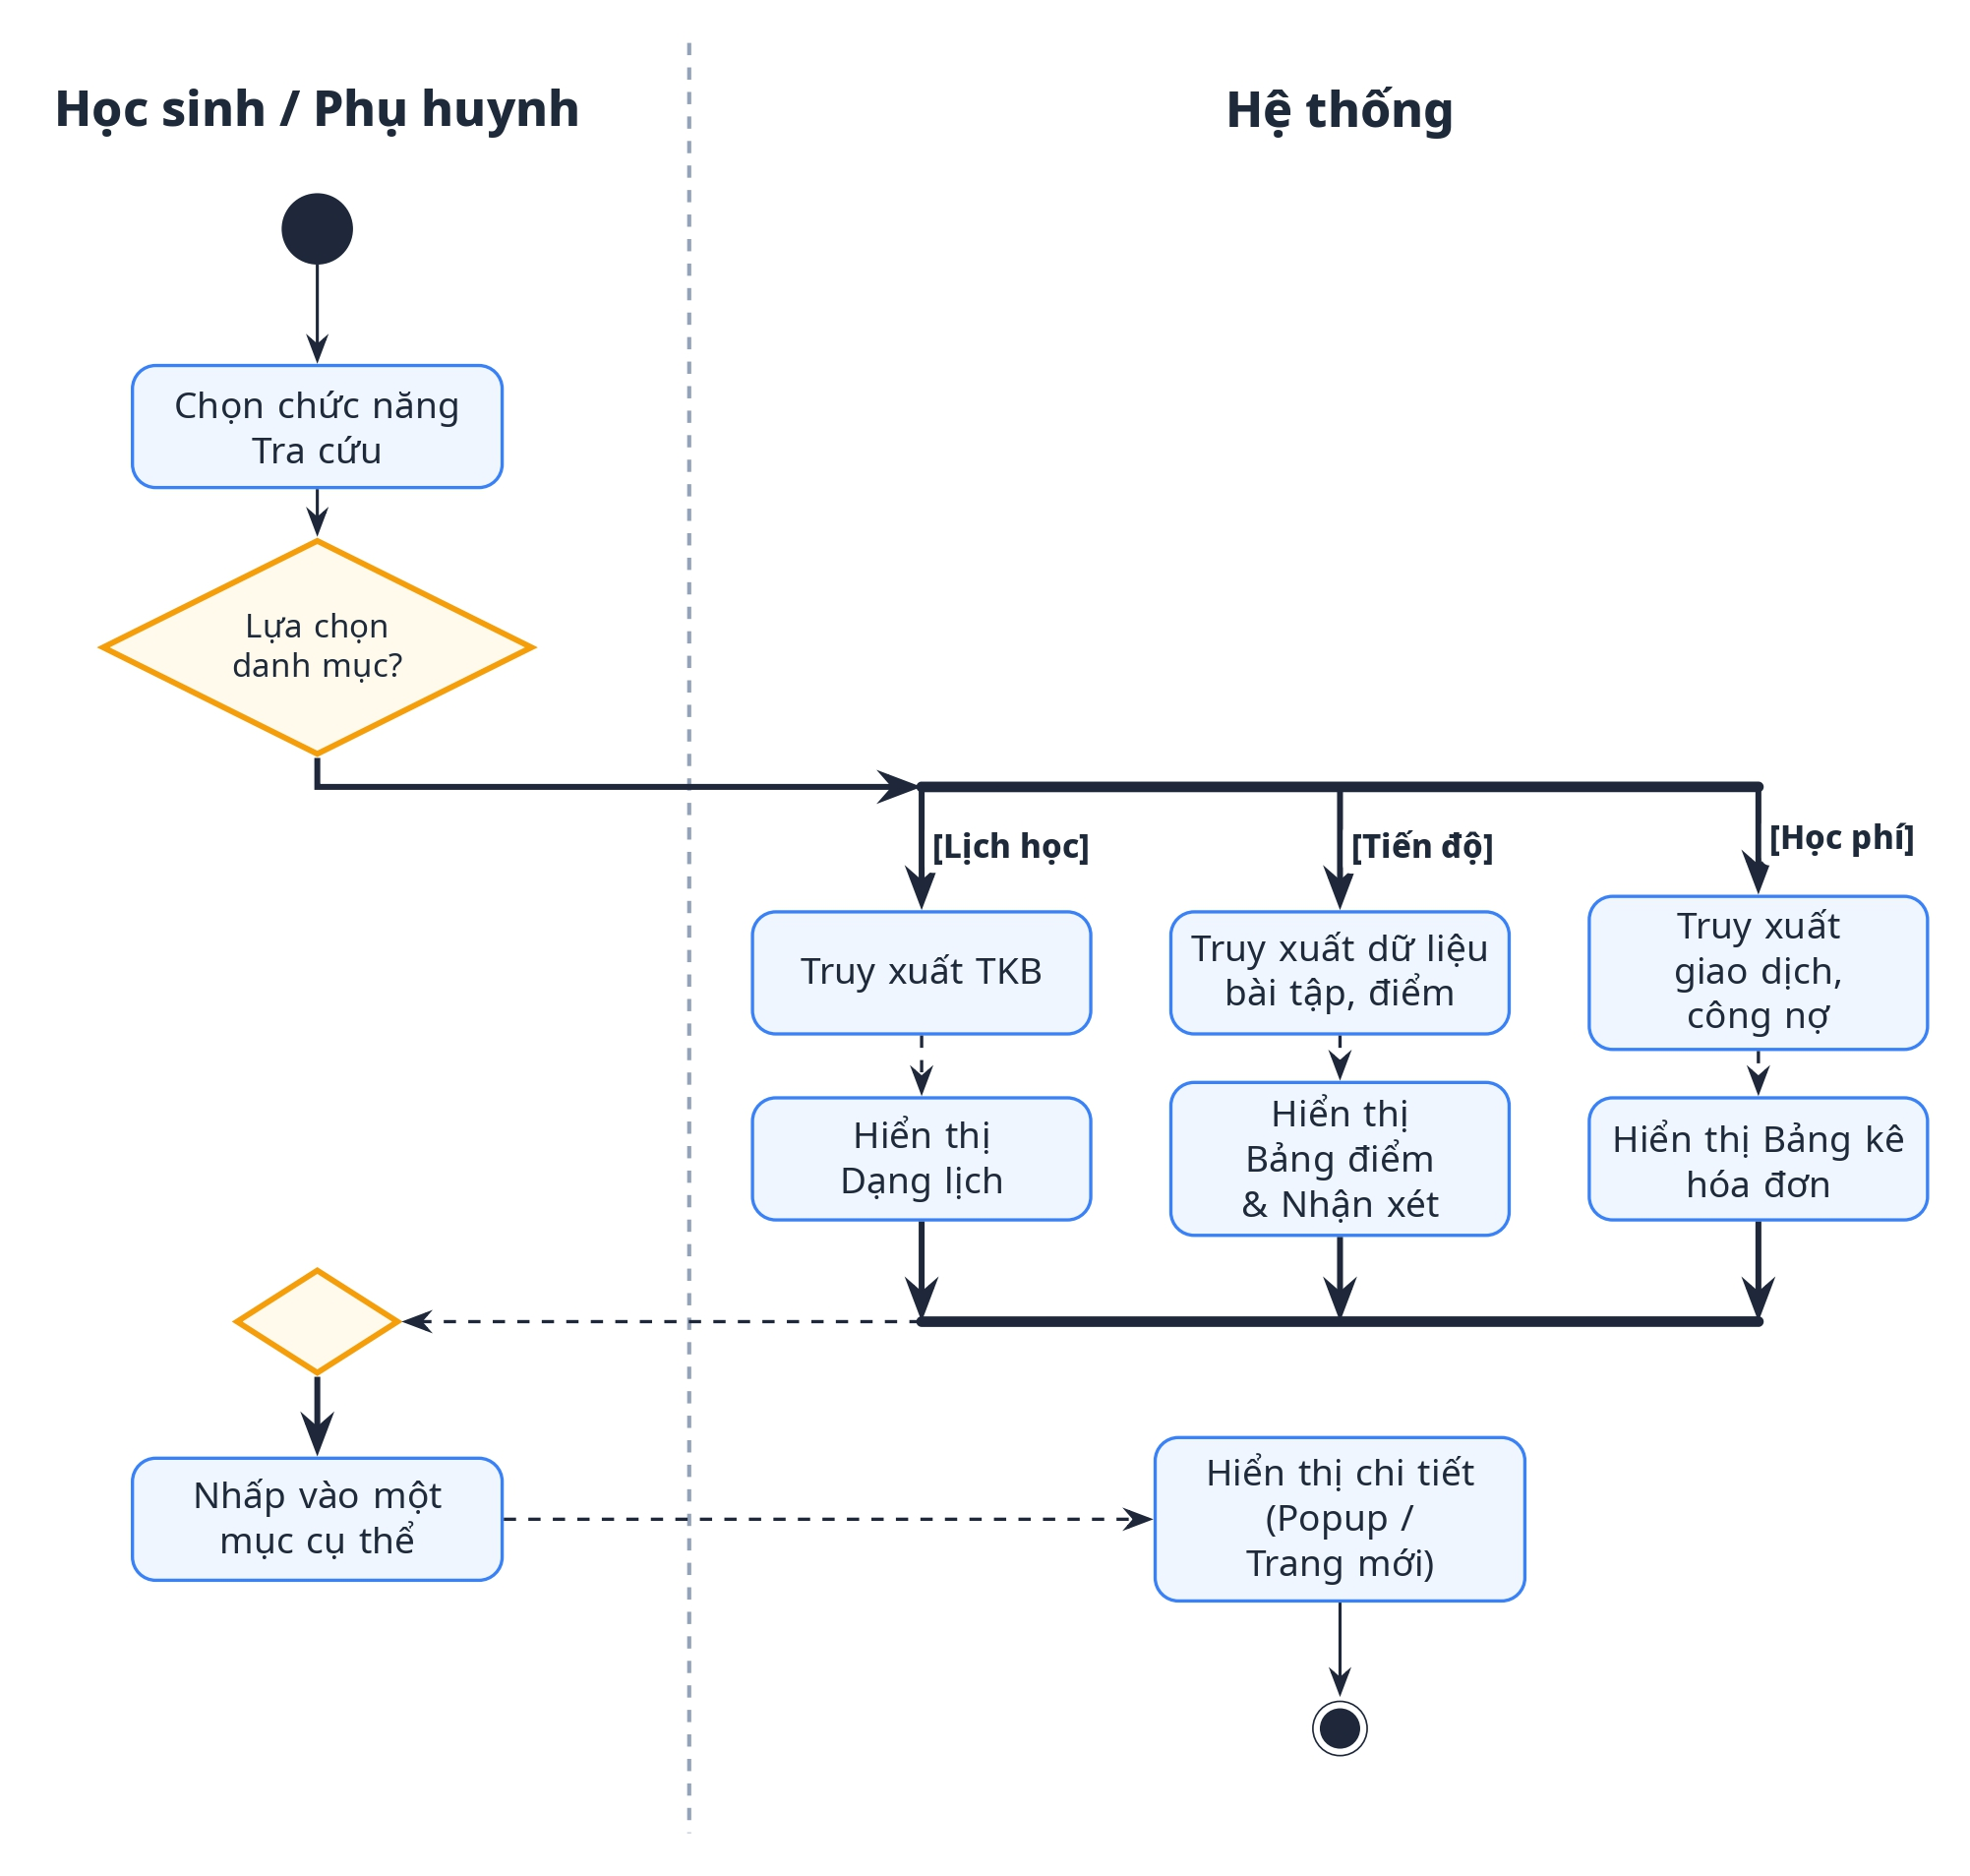
\includegraphics[width=0.8\textwidth]{picC2/AD7.jpg}
    \caption{AD-07: Quy trình Tra cứu thông tin}
\end{figure}

\clearpage
\section{Đặc tả use case}
\subsection{UC-01: Đăng nhập}

\begin{table}[htbp]
\centering
\small
\caption{Đặc tả Use Case UC-01: Đăng nhập}
\label{tab:uc01-dang-nhap}
\begin{tabularx}{\textwidth}{|>{\bfseries\raggedright\arraybackslash}p{2.5cm}|X|}
\hline
Đặc điểm & Nội dung \\ \hline
Mã \& Tên & UC-01 - Đăng nhập \\ \hline
Actor & Mọi Actor (Giáo viên, Học sinh, Phụ huynh) \\ \hline
Mục tiêu & Xác thực danh tính để truy cập vào hệ thống với quyền hạn tương ứng. \\ \hline
Tiền điều kiện & Người dùng đã có tài khoản trên hệ thống. \\ \hline
Luồng chính & 
\begin{enumerate}
    \item Người dùng truy cập trang đăng nhập.
    \item Người dùng nhập Tên đăng nhập và Mật khẩu.
    \item Nhấn nút "Đăng nhập".
    \item Hệ thống kiểm tra thông tin. Nếu hợp lệ, hệ thống cấp phiên làm việc và chuyển hướng đến Trang chủ (Dashboard) tương ứng với vai trò của người dùng.
\end{enumerate} \\ \hline
Luồng ngoại lệ & 
\begin{itemize}
    \item \textbf{Thông tin sai:} Hệ thống báo lỗi "Tài khoản hoặc mật khẩu không chính xác" và yêu cầu nhập lại.
\end{itemize} \\ \hline
\end{tabularx}
\end{table}

\subsection{UC-02: Quản lý người dùng \& phân quyền}

\begin{table}[htbp]
\centering
\small
\caption{Đặc tả Use Case UC-02: Quản lý người dùng \& phân quyền}
\label{tab:uc02-quan-ly-nguoi-dung}
\begin{tabularx}{\textwidth}{|>{\bfseries\raggedright\arraybackslash}p{2.5cm}|X|}
\hline
Đặc điểm & Nội dung \\ \hline
Mã \& Tên & UC-02 - Quản lý người dùng \& phân quyền \\ \hline
Actor & Giáo viên \\ \hline
Mục tiêu & Cấp phát và quản lý tài khoản truy cập cho Học sinh và Phụ huynh. \\ \hline
Luồng chính & 
\begin{enumerate}
    \item Giáo viên chọn "Quản lý người dùng".
    \item Chọn "Thêm mới tài khoản".
    \item Nhập thông tin (Họ tên, SĐT/Email) và chọn Vai trò (Học sinh / Phụ huynh).
    \item Nếu là Phụ huynh, hệ thống yêu cầu liên kết với tài khoản Học sinh đã có.
    \item Nhấn "Lưu". Hệ thống khởi tạo tài khoản, sinh mật khẩu mặc định và lưu vào cơ sở dữ liệu.
\end{enumerate} \\ \hline
\end{tabularx}
\end{table}
\clearpage
\subsection{UC-03: Quản lý lớp học}

\begin{table}[h!]
\centering
\small
\caption{Đặc tả Use Case UC-03: Quản lý lớp học}
\label{tab:uc03-quan-ly-lop-hoc}
\begin{tabularx}{\textwidth}{|>{\bfseries\raggedright\arraybackslash}p{2.5cm}|X|}
\hline
Đặc điểm & Nội dung \\ \hline
Mã \& Tên & UC-03 - Quản lý lớp học \\ \hline
Actor & Giáo viên \\ \hline
Mục tiêu & Cho phép giáo viên tạo mới, chỉnh sửa thông tin hoặc kết thúc (đóng) một lớp học/nhóm học. \\ \hline
Tiền điều kiện & Giáo viên đã đăng nhập vào hệ thống. \\ \hline
Luồng chính & 
\textbf{Tạo lớp học mới:}
\begin{enumerate}
    \item Giáo viên truy cập chức năng "Danh sách lớp học".
    \item Nhấn nút "Tạo lớp học mới".
    \item Nhập thông tin: Tên lớp, Môn học, Học phí cơ bản, Ngày bắt đầu.
    \item Nhấn "Lưu". Hệ thống kiểm tra hợp lệ và tạo lớp mới ở trạng thái "Đang hoạt động" với sĩ số ban đầu là 0.
\end{enumerate} \\ \hline
Luồng phụ & 
\textbf{1. Chỉnh sửa lớp học:}
\begin{enumerate}
    \item Tại "Danh sách lớp học", giáo viên chọn một lớp học đang có và nhấn "Chỉnh sửa".
    \item Hệ thống hiển thị biểu mẫu với các thông tin hiện tại của lớp.
    \item Giáo viên thay đổi các thông tin cần thiết (Tên lớp, Môn học, Học phí cơ bản, Mô tả...).
    \item Nhấn "Lưu". Hệ thống kiểm tra tính hợp lệ và cập nhật thông tin mới cho lớp học.
\end{enumerate}
\textbf{2. Kết thúc lớp học:}
\begin{enumerate}
    \item Tại "Danh sách lớp học", giáo viên chọn lớp học cần đóng và nhấn "Kết thúc lớp học".
    \item Hệ thống kiểm tra trạng thái lớp và hiển thị hộp thoại yêu cầu xác nhận.
    \item Giáo viên nhấn "Xác nhận".
    \item Hệ thống chuyển trạng thái lớp sang "Đã kết thúc", hủy các buổi học chưa diễn ra trong tương lai và ngừng phát sinh kỳ thu học phí mới (nhưng vẫn lưu trữ lịch sử điểm danh, điểm số và công nợ cũ để tra cứu).
\end{enumerate} \\ \hline
Luồng thay thế & 
\begin{itemize}
    \item \textbf{Còn công nợ khi kết thúc lớp:} Nếu lớp học còn hóa đơn học phí chưa thanh toán hết, hệ thống hiển thị cảnh báo danh sách học sinh còn nợ để giáo viên kiểm tra trước khi xác nhận đóng lớp.
\end{itemize} \\ \hline
Luồng ngoại lệ & 
\begin{itemize}
    \item \textbf{Dữ liệu không hợp lệ:} Khi tạo mới hoặc sửa, nếu bỏ trống thông tin bắt buộc hoặc nhập sai định dạng học phí, hệ thống báo lỗi và yêu cầu nhập lại.
\end{itemize} \\ \hline
\end{tabularx}
\end{table}

\clearpage
\subsection{UC-04: Lập thời khóa biểu}

\begin{table}[htbp]
\centering
\small
\caption{Đặc tả Use Case UC-04: Lập thời khóa biểu}
\label{tab:uc04-lap-thoi-khoa-bieu}
\begin{tabularx}{\textwidth}{|>{\bfseries\raggedright\arraybackslash}p{2.5cm}|X|}
\hline
Đặc điểm & Nội dung \\ \hline
Mã \& Tên & UC-04 - Lập thời khóa biểu \\ \hline
Actor & Giáo viên \\ \hline
Mục tiêu & Thiết lập lịch học định kỳ hoặc từng buổi cho lớp học. \\ \hline
Tiền điều kiện & Lớp học đã được tạo (UC-03). \\ \hline
Luồng chính & 
\begin{enumerate}
    \item Chọn lớp học cần lập lịch.
    \item Chọn "Thêm lịch học".
    \item Chọn Ngày, Giờ bắt đầu, Giờ kết thúc và Phòng học (hoặc Link học online).
    \item Chọn lặp lại (Hàng tuần) hoặc chỉ một buổi.
    \item Nhấn "Lưu". Hệ thống tự động sinh ra các buổi học vào danh sách.
\end{enumerate} \\ \hline
\end{tabularx}
\end{table}
\clearpage
\subsection{UC-05: Quản lý danh sách học sinh}

\begin{table}[h!]
\centering
\small
\caption{Đặc tả Use Case UC-05: Quản lý danh sách học sinh}
\label{tab:uc05-quan-ly-danh-sach-hoc-sinh}
\begin{tabularx}{\textwidth}{|>{\bfseries\raggedright\arraybackslash}p{2.5cm}|X|}
\hline
Đặc điểm & Nội dung \\ \hline
Mã \& Tên & UC-05 - Quản lý danh sách học sinh \\ \hline
Actor & Giáo viên \\ \hline
Mục tiêu & Thêm hoặc bớt (xóa/cho nghỉ) học sinh trong một lớp học cụ thể. \\ \hline
Tiền điều kiện & Lớp học đã được tạo (UC-03) và đang ở trạng thái hoạt động. \\ \hline
Luồng chính & 
\textbf{Thêm học sinh vào lớp:}
\begin{enumerate}
    \item Giáo viên mở trang chi tiết của lớp học cần quản lý.
    \item Chọn "Thêm học sinh". Hệ thống hiển thị danh sách các học sinh chưa có trong lớp.
    \item Giáo viên tìm kiếm, tích chọn các học sinh cần thêm và nhấn "Xác nhận".
    \item Hệ thống cập nhật tăng sĩ số lớp và tự động thêm lịch học của lớp vào thời khóa biểu của các học sinh đó.
\end{enumerate} \\ \hline
Luồng phụ & 
\textbf{Xóa học sinh khỏi lớp (Cho nghỉ học):}
\begin{enumerate}
    \item Giáo viên mở chi tiết lớp học và xem danh sách học sinh hiện tại của lớp.
    \item Chọn học sinh cần đưa ra khỏi lớp và nhấn "Xóa khỏi lớp" hoặc "Cho nghỉ học".
    \item Hệ thống hiển thị hộp thoại xác nhận (cho phép nhập ghi chú/lý do nghỉ nếu cần).
    \item Giáo viên nhấn "Xác nhận". Hệ thống chuyển trạng thái học sinh trong lớp sang "Đã nghỉ", giảm sĩ số hiện tại của lớp và gỡ các buổi học tương lai của lớp đó khỏi thời khóa biểu của học sinh (vẫn giữ nguyên lịch sử điểm danh, điểm số và học phí trước đó).
\end{enumerate} \\ \hline
Luồng thay thế & 
\begin{itemize}
    \item \textbf{Trùng lịch học (khi thêm):} Nếu lịch học của lớp trùng với một lớp khác mà học sinh đang theo học, hệ thống hiển thị cảnh báo cho giáo viên trước khi xác nhận.
    \item \textbf{Học sinh còn nợ học phí (khi bớt):} Hệ thống thông báo cho giáo viên biết các khoản phí chưa thanh toán của học sinh tại lớp này trước khi hoàn tất thao tác xóa khỏi danh sách đang học.
\end{itemize} \\ \hline
\end{tabularx}
\end{table}

\clearpage
\subsection{UC-06: Điểm danh}

\begin{table}[htbp]
\centering
\small
\caption{Đặc tả Use Case UC-06: Điểm danh}
\label{tab:uc06-diem-danh}
\begin{tabularx}{\textwidth}{|>{\bfseries\raggedright\arraybackslash}p{2.5cm}|X|}
\hline
Đặc điểm & Nội dung \\ \hline
Mã \& Tên & UC-06 - Điểm danh \\ \hline
Actor & Giáo viên \\ \hline
Mục tiêu & Ghi nhận trạng thái tham gia buổi học của từng học sinh. \\ \hline
Tiền điều kiện & Buổi học đã có trong lịch và danh sách lớp đã có học sinh. \\ \hline
Luồng chính & 
\begin{enumerate}
    \item Giáo viên chọn chức năng "Điểm danh" cho một buổi học trong ngày.
    \item Hệ thống hiển thị danh sách học sinh kèm trạng thái mặc định.
    \item Giáo viên đánh dấu trạng thái (Có mặt, Vắng, Trễ) cho từng học sinh.
    \item Giáo viên có thể nhập thêm ghi chú (nếu có).
    \item Nhấn "Lưu". Hệ thống lưu dữ liệu chuyên cần.
\end{enumerate} \\ \hline
\end{tabularx}
\end{table}

\subsection{UC-07: Quản lý bài tập và bài kiểm tra}

\begin{table}[htbp]
\centering
\small
\caption{Đặc tả Use Case UC-07: Quản lý bài tập và bài kiểm tra}
\label{tab:uc07-quan-ly-bai-tap}
\begin{tabularx}{\textwidth}{|>{\bfseries\raggedright\arraybackslash}p{2.5cm}|X|}
\hline
Đặc điểm & Nội dung \\ \hline
Mã \& Tên & UC-07 - Quản lý bài tập và bài kiểm tra \\ \hline
Actor & Giáo viên \\ \hline
Mục tiêu & Lên danh sách các bài kiểm tra đánh giá năng lực hoặc bài tập về nhà. \\ \hline
Luồng chính & 
\begin{enumerate}
    \item Giáo viên mở lớp học, chọn Tab "Bài tập/Kiểm tra".
    \item Nhấn "Tạo mới".
    \item Nhập Tên bài, Loại (BTVN / Thi giữa kỳ / Thi cuối kỳ), Ngày giao, Hạn chót.
    \item Nhấn "Lưu". Hệ thống tạo mục lưu trữ điểm số chờ nhập cho bài kiểm tra này.
\end{enumerate} \\ \hline
\end{tabularx}
\end{table}

\clearpage
\subsection{UC-08: Cập nhật điểm số}

\begin{table}[htbp]
\centering
\small
\caption{Đặc tả Use Case UC-08: Cập nhật điểm số}
\label{tab:uc08-cap-nhat-diem-so}
\begin{tabularx}{\textwidth}{|>{\bfseries\raggedright\arraybackslash}p{2.5cm}|X|}
\hline
Đặc điểm & Nội dung \\ \hline
Mã \& Tên & UC-08 - Cập nhật điểm số \\ \hline
Actor & Giáo viên \\ \hline
Mục tiêu & Nhập và lưu trữ điểm số, nhận xét cho học sinh. \\ \hline
Tiền điều kiện & Bài tập/Kiểm tra đã được tạo (UC-07). \\ \hline
Luồng chính & 
\begin{enumerate}
    \item Giáo viên chọn bài kiểm tra cần nhập điểm.
    \item Hệ thống hiển thị danh sách học sinh trong lớp.
    \item Giáo viên nhập điểm số và nhận xét chi tiết vào các ô tương ứng.
    \item Nhấn "Lưu điểm". Hệ thống cập nhật bảng điểm và ngay lập tức Học sinh/Phụ huynh có thể nhìn thấy.
\end{enumerate} \\ \hline
\end{tabularx}
\end{table}

\subsection{UC-09: Quản lý học phí}

\begin{table}[htbp]
\centering
\small
\caption{Đặc tả Use Case UC-09: Quản lý học phí}
\label{tab:uc09-quan-ly-hoc-phi}
\begin{tabularx}{\textwidth}{|>{\bfseries\raggedright\arraybackslash}p{2.5cm}|X|}
\hline
Đặc điểm & Nội dung \\ \hline
Mã \& Tên & UC-09 - Quản lý học phí \\ \hline
Actor & Giáo viên \\ \hline
Mục tiêu & Quản lý việc lập hóa đơn thu tiền và ghi nhận thanh toán. \\ \hline
Luồng chính & 
\begin{enumerate}
    \item Giáo viên chọn "Quản lý học phí" $\rightarrow$ Lập báo phí.
    \item Hệ thống tự động tính học phí dựa trên số buổi học và đơn giá.
    \item Giáo viên kiểm tra và "Phát hành" báo phí tới Phụ huynh.
    \item Khi Phụ huynh đóng tiền, Giáo viên tìm hóa đơn, nhập số tiền thực nhận.
    \item Hệ thống tự động cập nhật trạng thái (Đã đóng đủ / Còn nợ) dựa trên số tiền nhận.
\end{enumerate} \\ \hline
\end{tabularx}
\end{table}

\clearpage
\subsection{UC-10, 11, 12: Nhóm chức năng Tra cứu}

\begin{table}[htbp]
\centering
\small
\caption{Đặc tả Use Case UC-10, 11, 12: Nhóm chức năng Tra cứu}
\label{tab:uc10-11-12-tra-cuu}
\begin{tabularx}{\textwidth}{|>{\bfseries\raggedright\arraybackslash}p{2.5cm}|X|}
\hline
Đặc điểm & Nội dung \\ \hline
Mã \& Tên & UC-10, UC-11, UC-12 - Tra cứu Lịch học, Điểm số \& Học phí \\ \hline
Actor & Học sinh, Phụ huynh \\ \hline
Mục tiêu & Giúp người dùng biết thời gian học, theo dõi tiến độ và nắm bắt công nợ. \\ \hline
Luồng chính & 
\begin{enumerate}
    \item Người dùng đăng nhập và chọn danh mục cần tra cứu (Lịch học / Kết quả / Học phí).
    \item Hệ thống truy xuất dữ liệu liên quan đến hồ sơ của học sinh.
    \item Giao diện hiển thị chi tiết (Dạng lịch, Bảng điểm, hoặc Bảng kê hóa đơn).
    \item Người dùng có thể nhấp vào từng mục cụ thể để xem chi tiết thông tin.
\end{enumerate} \\ \hline
\end{tabularx}
\end{table}

\section{Các yêu cầu phi chức năng}
Bên cạnh các yêu cầu chức năng nghiệp vụ, phần mềm Hệ thống quản lý lớp học thêm còn phải tuân thủ các yêu cầu phi chức năng nhằm đảm bảo tính ổn định, độ an toàn và chất lượng vận hành của hệ thống. Trước hết về hiệu năng, hệ thống phải bảo đảm tốc độ xử lý nhanh chóng với thời gian phản hồi cho các thao tác cơ bản như tra cứu lịch học, xem điểm hay điểm danh trung bình dưới 3 giây. Đồng thời, hệ thống cần đáp ứng khả năng chịu tải ổn định cho khoảng 50 đến 100 người dùng truy cập đồng thời mà không xảy ra tình trạng gián đoạn. Trong quá trình thực hiện các chuỗi sự kiện của từng use case, nếu xảy ra sự cố
khi kết nối hoặc thao tác với cơ sở dữ liệu, hệ thống phải có cơ chế thông báo lỗi rõ ràng để người dùng phân biệt giữa lỗi hệ thống và lỗi nhập liệu. Các chức năng thuộc phạm vi của Giáo viên, Phụ huynh, Học sinh chỉ được thực hiện khi tác nhân đã đăng nhập đúng với vai trò tương ứng.

Về khả năng sử dụng, hệ thống cần có giao diện thân thiện và trực quan, cho phép người dùng dễ dàng tiếp cận các tính năng quan trọng. Các thao tác phải đơn giản, rõ
ràng và dễ thực hiện trên nhiều loại thiết bị khác nhau, từ máy tính cho đến điện thoại di động. Khi người dùng mắc lỗi trong quá trình thao tác, hệ thống phải hiển thị thông báo chi tiết để họ nhận biết vị trí lỗi, nguyên nhân gây lỗi và cách khắc phục, thay vì chỉ báo lỗi chung chung.

Về độ tin cậy và tính ổn định, hệ thống cần duy trì hoạt động liên tục 24 giờ mỗi ngày và 7 ngày mỗi tuần, với tỷ lệ ngừng hoạt động trong năm không vượt quá 5\%. Tất cả dữ liệu quan trọng của người dùng và sự kiện phải được lưu trữ an toàn, tránh thất thoát khi có sự cố.

Để hệ thống dễ dàng duy trì và phát triển lâu dài, yêu cầu về tính dễ bảo trì cũng phải được đáp ứng. Kiến trúc phần mềm cần được thiết kế theo hướng module hóa, giúp việc sửa lỗi, nâng cấp và mở rộng tính năng trở nên thuận tiện. Mã nguồn phải được lưu trữ và quản lý trên các nền tảng kiểm soát phiên bản GitHub, đi kèm với tài liệu kỹ thuật và hướng dẫn triển khai chi tiết để đội ngũ phát triển hoặc vận hành có thể tiếp quản dễ dàng.

Cuối cùng, yêu cầu về an toàn và bảo mật phải được đặt lên hàng đầu. Quyền truy cập phải được phân chia rõ ràng theo từng vai trò, tránh tình trạng người dùng thông thường có
thể truy cập vào các chức năng của Giáo viên.